
%% bare_conf.tex
%% V1.4b
%% 2015/08/26
%% by Michael Shell
%% See:
%% http://www.michaelshell.org/
%% for current contact information.
%%
%% This is a skeleton file demonstrating the use of IEEEtran.cls
%% (requires IEEEtran.cls version 1.8b or later) with an IEEE
%% conference paper.
%%
%% Support sites:
%% http://www.michaelshell.org/tex/ieeetran/
%% http://www.ctan.org/pkg/ieeetran
%% and
%% http://www.ieee.org/

%%*************************************************************************
%% Legal Notice:
%% This code is offered as-is without any warranty either expressed or
%% implied; without even the implied warranty of MERCHANTABILITY or
%% FITNESS FOR A PARTICULAR PURPOSE! 
%% User assumes all risk.
%% In no event shall the IEEE or any contributor to this code be liable for
%% any damages or losses, including, but not limited to, incidental,
%% consequential, or any other damages, resulting from the use or misuse
%% of any information contained here.
%%
%% All comments are the opinions of their respective authors and are not
%% necessarily endorsed by the IEEE.
%%
%% This work is distributed under the LaTeX Project Public License (LPPL)
%% ( http://www.latex-project.org/ ) version 1.3, and may be freely used,
%% distributed and modified. A copy of the LPPL, version 1.3, is included
%% in the base LaTeX documentation of all distributions of LaTeX released
%% 2003/12/01 or later.
%% Retain all contribution notices and credits.
%% ** Modified files should be clearly indicated as such, including  **
%% ** renaming them and changing author support contact information. **
%%*************************************************************************


% *** Authors should verify (and, if needed, correct) their LaTeX system  ***
% *** with the testflow diagnostic prior to trusting their LaTeX platform ***
% *** with production work. The IEEE's font choices and paper sizes can   ***
% *** trigger bugs that do not appear when using other class files.       ***                          ***
% The testflow support page is at:
% http://www.michaelshell.org/tex/testflow/



\documentclass[conference]{IEEEtran}
% Some Computer Society conferences also require the compsoc mode option,
% but others use the standard conference format.
%
% If IEEEtran.cls has not been installed into the LaTeX system files,
% manually specify the path to it like:
% \documentclass[conference]{../sty/IEEEtran}





% Some very useful LaTeX packages include:
% (uncomment the ones you want to load)


% *** MISC UTILITY PACKAGES ***
%
%\usepackage{ifpdf}
% Heiko Oberdiek's ifpdf.sty is very useful if you need conditional
% compilation based on whether the output is pdf or dvi.
% usage:
% \ifpdf
%   % pdf code
% \else
%   % dvi code
% \fi
% The latest version of ifpdf.sty can be obtained from:
% http://www.ctan.org/pkg/ifpdf
% Also, note that IEEEtran.cls V1.7 and later provides a builtin
% \ifCLASSINFOpdf conditional that works the same way.
% When switching from latex to pdflatex and vice-versa, the compiler may
% have to be run twice to clear warning/error messages.






% *** CITATION PACKAGES ***
%
%\usepackage{cite}
% cite.sty was written by Donald Arseneau
% V1.6 and later of IEEEtran pre-defines the format of the cite.sty package
% \cite{} output to follow that of the IEEE. Loading the cite package will
% result in citation numbers being automatically sorted and properly
% "compressed/ranged". e.g., [1], [9], [2], [7], [5], [6] without using
% cite.sty will become [1], [2], [5]--[7], [9] using cite.sty. cite.sty's
% \cite will automatically add leading space, if needed. Use cite.sty's
% noadjust option (cite.sty V3.8 and later) if you want to turn this off
% such as if a citation ever needs to be enclosed in parenthesis.
% cite.sty is already installed on most LaTeX systems. Be sure and use
% version 5.0 (2009-03-20) and later if using hyperref.sty.
% The latest version can be obtained at:
% http://www.ctan.org/pkg/cite
% The documentation is contained in the cite.sty file itself.






% *** GRAPHICS RELATED PACKAGES ***
%
\ifCLASSINFOpdf
  % \usepackage[pdftex]{graphicx}
  % declare the path(s) where your graphic files are
  % \graphicspath{{../pdf/}{../jpeg/}}
  % and their extensions so you won't have to specify these with
  % every instance of \includegraphics
  % \DeclareGraphicsExtensions{.pdf,.jpeg,.png}
\else
  % or other class option (dvipsone, dvipdf, if not using dvips). graphicx
  % will default to the driver specified in the system graphics.cfg if no
  % driver is specified.
  \usepackage[dvips]{graphicx}
  % declare the path(s) where your graphic files are
  \graphicspath{{./figures/}{./eps/}}
  % and their extensions so you won't have to specify these with
  % every instance of \includegraphics
  \DeclareGraphicsExtensions{.eps}
\fi
% graphicx was written by David Carlisle and Sebastian Rahtz. It is
% required if you want graphics, photos, etc. graphicx.sty is already
% installed on most LaTeX systems. The latest version and documentation
% can be obtained at: 
% http://www.ctan.org/pkg/graphicx
% Another good source of documentation is "Using Imported Graphics in
% LaTeX2e" by Keith Reckdahl which can be found at:
% http://www.ctan.org/pkg/epslatex
%
% latex, and pdflatex in dvi mode, support graphics in encapsulated
% postscript (.eps) format. pdflatex in pdf mode supports graphics
% in .pdf, .jpeg, .png and .mps (metapost) formats. Users should ensure
% that all non-photo figures use a vector format (.eps, .pdf, .mps) and
% not a bitmapped formats (.jpeg, .png). The IEEE frowns on bitmapped formats
% which can result in "jaggedy"/blurry rendering of lines and letters as
% well as large increases in file sizes.
%
% You can find documentation about the pdfTeX application at:
% http://www.tug.org/applications/pdftex





% *** MATH PACKAGES ***
%
%\usepackage{amsmath}
% A popular package from the American Mathematical Society that provides
% many useful and powerful commands for dealing with mathematics.
%
% Note that the amsmath package sets \interdisplaylinepenalty to 10000
% thus preventing page breaks from occurring within multiline equations. Use:
%\interdisplaylinepenalty=2500
% after loading amsmath to restore such page breaks as IEEEtran.cls normally
% does. amsmath.sty is already installed on most LaTeX systems. The latest
% version and documentation can be obtained at:
% http://www.ctan.org/pkg/amsmath





% *** SPECIALIZED LIST PACKAGES ***
%
%\usepackage{algorithmic}
% algorithmic.sty was written by Peter Williams and Rogerio Brito.
% This package provides an algorithmic environment fo describing algorithms.
% You can use the algorithmic environment in-text or within a figure
% environment to provide for a floating algorithm. Do NOT use the algorithm
% floating environment provided by algorithm.sty (by the same authors) or
% algorithm2e.sty (by Christophe Fiorio) as the IEEE does not use dedicated
% algorithm float types and packages that provide these will not provide
% correct IEEE style captions. The latest version and documentation of
% algorithmic.sty can be obtained at:
% http://www.ctan.org/pkg/algorithms
% Also of interest may be the (relatively newer and more customizable)
% algorithmicx.sty package by Szasz Janos:
% http://www.ctan.org/pkg/algorithmicx




% *** ALIGNMENT PACKAGES ***
%
%\usepackage{array}
% Frank Mittelbach's and David Carlisle's array.sty patches and improves
% the standard LaTeX2e array and tabular environments to provide better
% appearance and additional user controls. As the default LaTeX2e table
% generation code is lacking to the point of almost being broken with
% respect to the quality of the end results, all users are strongly
% advised to use an enhanced (at the very least that provided by array.sty)
% set of table tools. array.sty is already installed on most systems. The
% latest version and documentation can be obtained at:
% http://www.ctan.org/pkg/array


% IEEEtran contains the IEEEeqnarray family of commands that can be used to
% generate multiline equations as well as matrices, tables, etc., of high
% quality.




% *** SUBFIGURE PACKAGES ***
%\ifCLASSOPTIONcompsoc
%  \usepackage[caption=false,font=normalsize,labelfont=sf,textfont=sf]{subfig}
%\else
%  \usepackage[caption=false,font=footnotesize]{subfig}
%\fi
% subfig.sty, written by Steven Douglas Cochran, is the modern replacement
% for subfigure.sty, the latter of which is no longer maintained and is
% incompatible with some LaTeX packages including fixltx2e. However,
% subfig.sty requires and automatically loads Axel Sommerfeldt's caption.sty
% which will override IEEEtran.cls' handling of captions and this will result
% in non-IEEE style figure/table captions. To prevent this problem, be sure
% and invoke subfig.sty's "caption=false" package option (available since
% subfig.sty version 1.3, 2005/06/28) as this is will preserve IEEEtran.cls
% handling of captions.
% Note that the Computer Society format requires a larger sans serif font
% than the serif footnote size font used in traditional IEEE formatting
% and thus the need to invoke different subfig.sty package options depending
% on whether compsoc mode has been enabled.
%
% The latest version and documentation of subfig.sty can be obtained at:
% http://www.ctan.org/pkg/subfig




% *** FLOAT PACKAGES ***
%
%\usepackage{fixltx2e}
% fixltx2e, the successor to the earlier fix2col.sty, was written by
% Frank Mittelbach and David Carlisle. This package corrects a few problems
% in the LaTeX2e kernel, the most notable of which is that in current
% LaTeX2e releases, the ordering of single and double column floats is not
% guaranteed to be preserved. Thus, an unpatched LaTeX2e can allow a
% single column figure to be placed prior to an earlier double column
% figure.
% Be aware that LaTeX2e kernels dated 2015 and later have fixltx2e.sty's
% corrections already built into the system in which case a warning will
% be issued if an attempt is made to load fixltx2e.sty as it is no longer
% needed.
% The latest version and documentation can be found at:
% http://www.ctan.org/pkg/fixltx2e


%\usepackage{stfloats}
% stfloats.sty was written by Sigitas Tolusis. This package gives LaTeX2e
% the ability to do double column floats at the bottom of the page as well
% as the top. (e.g., "\begin{figure*}[!b]" is not normally possible in
% LaTeX2e). It also provides a command:
%\fnbelowfloat
% to enable the placement of footnotes below bottom floats (the standard
% LaTeX2e kernel puts them above bottom floats). This is an invasive package
% which rewrites many portions of the LaTeX2e float routines. It may not work
% with other packages that modify the LaTeX2e float routines. The latest
% version and documentation can be obtained at:
% http://www.ctan.org/pkg/stfloats
% Do not use the stfloats baselinefloat ability as the IEEE does not allow
% \baselineskip to stretch. Authors submitting work to the IEEE should note
% that the IEEE rarely uses double column equations and that authors should try
% to avoid such use. Do not be tempted to use the cuted.sty or midfloat.sty
% packages (also by Sigitas Tolusis) as the IEEE does not format its papers in
% such ways.
% Do not attempt to use stfloats with fixltx2e as they are incompatible.
% Instead, use Morten Hogholm'a dblfloatfix which combines the features
% of both fixltx2e and stfloats:
%
% \usepackage{dblfloatfix}
% The latest version can be found at:
% http://www.ctan.org/pkg/dblfloatfix




% *** PDF, URL AND HYPERLINK PACKAGES ***
%
%\usepackage{url}
% url.sty was written by Donald Arseneau. It provides better support for
% handling and breaking URLs. url.sty is already installed on most LaTeX
% systems. The latest version and documentation can be obtained at:
% http://www.ctan.org/pkg/url
% Basically, \url{my_url_here}.




% *** Do not adjust lengths that control margins, column widths, etc. ***
% *** Do not use packages that alter fonts (such as pslatex).         ***
% There should be no need to do such things with IEEEtran.cls V1.6 and later.
% (Unless specifically asked to do so by the journal or conference you plan
% to submit to, of course. )


%
% PACKAGES
%
\usepackage{etoolbox}
\usepackage{units}
%\usepackage{graphicx} % STOP commenting this in and upload EPS
\usepackage{microtype}
\usepackage{hyperref}
\usepackage{breakurl}
\usepackage{comment} % TODO remove later
%
\usepackage[ruled,vlined]{algorithm2e}
\DontPrintSemicolon
\SetAlFnt{\scriptsize}
%
\newtoggle{doubleblind}
%\toggletrue{doubleblind}
\togglefalse{doubleblind}
%
\newtoggle{includeappendix}
\toggletrue{includeappendix}
%\togglefalse{includeappendix}
%
\newtoggle{includeacknowl}
%\toggletrue{includeacknowl}
\togglefalse{includeacknowl}
%
\usepackage[table,xcdraw]{xcolor}
%\usepackage{booktabs}
%
% NEW COMMANDS
%
\newcommand{\struc}[1]{\textcolor{blue}{ToWrite: #1 \\}}
\newcommand{\todo}[1]{\textcolor{red}{TODO: #1}}
\newcommand{\cJD}[1]{\textcolor{red}{\small{FIX: #1}}}
\newcommand{\rC}[0]{\rowcolor[HTML]{CCCCCC}}
\newcommand{\hC}[0]{\rowcolor[HTML]{333333}}
\newcommand{\tH}[1]{\multicolumn{1}{c}{\textcolor{white}{#1}}}

\makeatletter
\patchcmd{\@setref}{\bfseries ??}{\colorbox{red}{?r?}}{}{}
\patchcmd{\@citex}{\bfseries ?}{\colorbox{red}{?c?}}{}{}
\renewcommand{\algorithmcfname}{PseudoCode}
\makeatother


% correct bad hyphenation here
\hyphenation{op-tical net-works semi-conduc-tor}


\begin{document}
\iftoggle{highlightChanges}{
    \begin{titlepage}
    \mbox{}\\{\Large \textbf{Cover Letter for Submission:}\\\\Double-precision FPUs in High-Performance Computing: an Embarrassment of Riches?}
    \newline\newline\newline\newline\large
    Summary of the implemented changes (also highlighted in blue on subsequent pages):
    \begin{itemize}
        \item Added discussion of why we report flop/s and why it is necessary in this paper
        despite our later recommendation that the HPC community should not (only) report flop/s;
        \item Split of Fig.~\ref{fig:flops} (rel./abs. flop/s comparison) into two subfigures for
        easier readability and modification of text in Sec.~\ref{ssec:eval_flops} to reflect the
        change;
        \item Added Fig.~\ref{fig:t2s-rel} for ``Time-to-Solution'' and its explanation/discussion
        in Sec.~\ref{ssec:eval_flops};
        \item Added roofline analysis in Sec.~\ref{ssec:eval_roof} to determine the optimization
        status of the FP-intensive proxy-apps, which we used for this study (incl 2 additional
        references for this part)
        \item Added details about the theoretical peak speedup with turbo boost shown in
        Fig.~\ref{fig:freq} and explanation of why a pessimistic +100Mhz was chosen in this case
        and why this resulted in ``superlinear speedup'' for some benchmarks
        \item Added acknowledgement of funding resources and author's contributions;
        \item Added note to Tab.~\ref{table:rest} to point out the multiuse of two columns by
        similar metrics (VTune reports slightly different metrics for BDW vs. KNM/KNL for
        arithmetic intensity and memory-boundedness; and readers can consult Ref. [41] for an
        in-depth documentation on these metrics (as stated previously in the table's caption));
        \item (+ multiple smaller grammar and text adjustments which will no be highlighted).
    \end{itemize}
    \end{titlepage}
}{}
%%%% DONT TOUCH FOR DRAFT => TODO take out if we buy 1 page 
\bstctlcite{IEEEexample:BSTcontrol}
%%%% DONT TOUCH FOR DRAFT

%
% paper title
% Titles are generally capitalized except for words such as a, an, and, as,
% at, but, by, for, in, nor, of, on, or, the, to and up, which are usually
% not capitalized unless they are the first or last word of the title.
% Linebreaks \\ can be used within to get better formatting as desired.
% Do not put math or special symbols in the title.
%\title{Less FP64 Units for Everyone: Investigating the Impact of Having Less Double Precision FPUs on Processors for HPC Applications}
%\title{Bottlenecks in Modern Systems: Studying the Impact of FP64 Units on HPC Workloads}
\title{Double-precision FPUs in High-Performance Computing: an Embarrassment of Riches?}
%\cJD{All: add suggested commented better titles if you have any}}
%%Alternative titles 
%Busting the FLOPS Myth: The Relevance of FP64 Units to HPC Workloads
%Studying the Impact of FP64 Units on HPC Workloads


% author names and affiliations
% use a multiple column layout for up to three different
% affiliation
\iftoggle{doubleblind}{
  \author{(hidden for double-blind review)}
}{
  \author{
    \IEEEauthorblockN{
  Jens Domke\IEEEauthorrefmark{1},
  Kazuaki Matsumura\IEEEauthorrefmark{2},
  Mohamed Wahib\IEEEauthorrefmark{3},
%  Hamid R. Zohouri\IEEEauthorrefmark{2},\\
  Haoyu Zhang\IEEEauthorrefmark{2},
  Keita Yashima\IEEEauthorrefmark{2},\\
  Toshiki Tsuchikawa\IEEEauthorrefmark{2},
  Yohei Tsuji\IEEEauthorrefmark{2},
%  Ryan Barton\IEEEauthorrefmark{2},
  Artur Podobas\IEEEauthorrefmark{2},
  Satoshi Matsuoka\IEEEauthorrefmark{4}\textsuperscript{,}\IEEEauthorrefmark{2}
}
\\
\IEEEauthorblockA{\IEEEauthorrefmark{1}Global Scientific Information and Computing Center, Tokyo Institute of Technology}
\IEEEauthorblockA{\IEEEauthorrefmark{2}Department of Mathematical and Computing Science, Tokyo Institute of Technology}
\IEEEauthorblockA{\IEEEauthorrefmark{3}AIST-TokyoTech Real World Big-Data Computation Open Innovation Laboratory, Tokyo, Japan}
\IEEEauthorblockA{\IEEEauthorrefmark{4}RIKEN Center for Computational Science (R-CCS), RIKEN, Japan}

  }
}

% conference papers do not typically use \thanks and this command
% is locked out in conference mode. If really needed, such as for
% the acknowledgment of grants, issue a \IEEEoverridecommandlockouts
% after \documentclass

% for over three affiliations, or if they all won't fit within the width
% of the page, use this alternative format:
% 
%\author{\IEEEauthorblockN{Michael Shell\IEEEauthorrefmark{1},
%Homer Simpson\IEEEauthorrefmark{2},
%James Kirk\IEEEauthorrefmark{3}, 
%Montgomery Scott\IEEEauthorrefmark{3} and
%Eldon Tyrell\IEEEauthorrefmark{4}}
%\IEEEauthorblockA{\IEEEauthorrefmark{1}School of Electrical and Computer Engineering\\
%Georgia Institute of Technology,
%Atlanta, Georgia 30332--0250\\ Email: see http://www.michaelshell.org/contact.html}
%\IEEEauthorblockA{\IEEEauthorrefmark{2}Twentieth Century Fox, Springfield, USA\\
%Email: homer@thesimpsons.com}
%\IEEEauthorblockA{\IEEEauthorrefmark{3}Starfleet Academy, San Francisco, California 96678-2391\\
%Telephone: (800) 555--1212, Fax: (888) 555--1212}
%\IEEEauthorblockA{\IEEEauthorrefmark{4}Tyrell Inc., 123 Replicant Street, Los Angeles, California 90210--4321}}




% use for special paper notices
%\IEEEspecialpapernotice{(Invited Paper)}




% make the title area
\maketitle

% As a general rule, do not put math, special symbols or citations
% in the abstract
%\begin{abstract}
%The abstract goes here.
%\end{abstract}
% IPDPS requirement !Abstract (Maximum 250 words)!
\begin{abstract}
Among the (uncontended) common wisdoms in High-Performance Computing (HPC) is the applications’ need for large amount of double-precision support in hardware.  Hardware manufacturers, the TOP500 list, and (rarely revisited) legacy software have without doubt followed and contributed to this~view. 

In this paper, we challenge that wisdom, and we do so by exhaustively comparing a large number of HPC proxy application on two processors: Intel’s Knights Landing (KNL) and Knights Mill (KNM). Although similar, the KNM and KNL architecturally deviate at one important point: the silicon area devoted to double-precision arithmetic’s. This fortunate discrepancy allows us to empirically quantify the performance impact in reducing the amount of hardware double-precision arithmetic. %this part reads strange

Our analysis shows that this common wisdom might not always be right. We find that the investigated HPC proxy applications do allow for a (significant) reduction in double-precision with little-to-no performance implications. With the advent of a failing of Moore's law, our results partially reinforce the view taken by modern industry (e.g. upcoming ARM64FX) to trade double-precision silicon for hybrid-precision and/or bandwidth.

%\cJD{PLACEHOLDER: (Maximum 250 words)!}
%Common perception in supercomputing is that double precision floating point
%calculations is what matters, with respect to both application requirements and
%performance. Accordingly, chip manufacturers have allocated a significant
%portion of chip area to double precision FPUs, in turn reducing the chip's
%compute-per-silicon ratio, and also the bandwidth utilization.
%We conduct an exhaustive FPU-requirement and performance study using 22 HPC
%(proxy/mini) applications from various scientific domains, which comprise the
%majority of CPU cycles in HPC. These applications will be executed on two
%target platforms with overall similar characteristic, however drastically
%different amount of double precision units. Hence, this comparison will give
%vendors and the rest of the community a chance to investigate the precision
%or unit requirements, and identify performance bottlenecks in modern HPC codes,
%to guide the procurement towards more/less FP64, FP32, ..., or faster/bigger
%memory and caches, or more cores instead.
%\cJD{PLACEHOLDER: (Maximum 250 words)!}
\end{abstract}


% no keywords




% For peer review papers, you can put extra information on the cover
% page as needed:
% \ifCLASSOPTIONpeerreview
% \begin{center} \bfseries EDICS Category: 3-BBND \end{center}
% \fi
%
% For peerreview papers, this IEEEtran command inserts a page break and
% creates the second title. It will be ignored for other modes.
\IEEEpeerreviewmaketitle

% list of venues:
%  - ** IPDPS (~sep)
%  - * PPoPP (~aug)
%  - TACO (journal)
%  - TPDS (journal)
%  - JPDC (journal)
%  - CCgrid (~nov)
%  - (SC Asia)
%  - (HPC Asia)

% need: 1 full script setting up all -> for reproduce
%
% ignore post-K for now
%
% overall story:
%   - analyze apps-per-system overview (to guide purchase process, RFPs) + some hpc systems are 1-app only
%   - option a: rigor performance model; run on many (2-3) systems to see what happens if the next-gen comes (so, based on current info in apps, how are they expected to run on post-k or coral 1)
%   - option b: design a better flow/approach how to choose/design the next system
%   - option c: how to actually determine if app is compute or memory bound; we tried multiple ways, vtune, pcm, freq scaling
%   - option d: do we really need that much fp64? -> next study?
%   - ** option e: check which of our apps use high percentage of systems (>80%) and then give guide how to balance compute/network/memory for this use-case
%   - option f: compare time to solution for xeon/knl/knm and see the trend, not that much fp64 needed since knl with half fp64 performs roughly equivalent to knm
%   - ** option g: focus on time-to-solution (e.g. normalize run time / time-to-solution by memory bandwidth) and (maybe power -> not important for big players unless constrained building/power plant next door; they have gov/scientists to pay the bill)
%   - option h: code is fp64 -> we need fp64-heavy systems -> perf goes up is a WRONG graph: break at code -> architecture design
%   - option i: knm now real advantage over knm for our use case, so safe power and money to get near similar time-to-solution
%   - option j: We have empiric evidence that zealously allocating silicon to DP is unwise and it might be high time to revice how silicon is distributed.

\section{Introduction}\label{sec:intro}
% goal: 1 page
% - analyze if either of the BM suits has been used in other studies (not as individual apps but as the entire ECP/portK set
% - analyze the usage of what type of apps/sciences is run on HPC systems -> give weights on the apps and requirements

%\todo{==========GUIDE LINES=========\\}
%\todo{everyone make heavy use of cross-ref to sections and figs\\}
%\todo{write clear, short (~1/3 of a half-side) paragraphs, short sentences, "we" and "active" form!\\}
%\todo{never use abbreviations unless previously written somewhere like "...Knights Mill (KNM)..."\\}
%\todo{every fact, statement: BACK IT UP by cross-ref in this paper, ref to other
%papers/books/write-papers/manuals(/blogs/websites), or proof it otherwise\\}
%\todo{avoid "fancy" writing such as: fantastic, great, extreme high, poor, ...\\}
%\todo{please use newlines after 70--100 characters and not one or multiple sentences on single line\\}
%\todo{don't delete large sections of your writing; NEVER delete section of others; use \% to comment stuff
%out and notify the person\\}
%\todo{make heavy use of \textbackslash label and \textbackslash ref command for figs, tables, sections,
%subsections, equations, etc\\}

It is becoming increasingly clear that the road forward in High-Performance Computing (HPC) is one full of obstacles.
With the ending of Dennard's scaling~\cite{dennard_design_1974} and the ending of Moore's law~\cite{moore_lithography_1995},
there is today an ever-increasing need to oversee how we allocate the silicon to various functional units in modern many-core
processors. Amongst those decisions is how we distributed the hardware support for various levels of compute-precision.

Historically, most of the compute silicon has been allocated to double-precision (64-bit) compute.
Nowadays -- in processors such as the forthcoming AA64FX~\cite{yoshida_fujitsu_2018} and Nvidia
Volta~\cite{choquette_volta:_2018} -- the trend, mostly driven by market/AI demands, is to replace
some of the double-precision units with lower-precision units.
Lower-precision units occupy less area (up to $\approx$3x going from double- to single-precision
Fused-Multiply-Accumulate~\cite{pu_fpmax:_2016}), leading to more on-chip resources (more
instruction-level parallelism), potentially lowered energy consumption, and a definitive
decrease in external memory bandwidth pressure (i.e., more values per unit bandwidth).
The gains -- up to four times over their DP variants with little loss in
accuracy~\cite{haidar_harnessing_2018} -- are attractive and clear, but what is the impact on
performance (if any) on existing HPC applications? What performance impact can HPC users expect when migrating their code to future processors with a different distribution
in floating-point precision support? Finally, how can we empirically quantify this impact on
performance using existing processors in an apples-to-apples comparison on real-life use cases
without relying on tedious, slow, and potentially inaccurate simulators? %\cJD{note: make sure we actually will answer these}

The Intel Xeon Phi was supposed to be the high-end for many-core processor technology for nearly
a decade (Knights Ferry was announced in 2010), and has changed drastically since its first released.
The latest (and also last) two revisions -- the Knights Landing and Knights Mill -- are of
particular importance since they arguable reflect two different ways of thinking. Knights Landing
has relatively large support for double-precision (64-bit) computations, and follows a
more traditional school of thought. The Knights Mill follows a different direction, which is the replacement
of double-precision compute units with lower-precision (single-precision, half-precision, and integer)
compute capabilities.

In the present paper, we quantify and analyze the performance and compute bottlenecks of
Intel's Knights Landing~\cite{sodani_knights_2016} and Mill architectures~\cite{bradford_knights_2017} -- two
processors with identical micro-architecture where the main difference is in the relative allocation of double-precision units.
We stress both processors with numerous realistic benchmarks from both the
Exascale Computing Project (ECP) proxy applications~\cite{noauthor_ecp_2018} and
RIKEN-CCS Fiber Miniapp Suite~\cite{riken_aics_fiber_2015} -- benchmarks used in HPC system acquisition.
Through an extensive (and robust) performance measurement process (which we also open-source), we
empirically show the architecture's relative weaknesses. In short, the contributions of the present paper are:
\begin{enumerate}
    \item An empirical performance evaluation of the Knights Landing and Mill family of processors -- both proxies for previous and future architectural trends -- with respect to benchmarks derived from realistic HPC workloads,
    \item  An in-depth analysis of results, including identification of bottlenecks for the different application/architecture combinations, and
    \item An open-source compilation of our evaluation methodology, including our collected raw data.
    %including experience and fallacies encountered, revealing gaps in state-of-the-art profiling tools and debuggers (including their work-around).
\end{enumerate}
%
%\cJD{if possible include some small figure as result teaser}
%
%The remaining paper is organized as follows: \textbf{Artur: TODO. Likely will omitt.}\cJD{yes, omit}.
%% OLD TEXT BELOW. COMMENTED OUT BY ARTUR
%Common wisdom in HPC is that double precision floating point calculations is what matters, with respect to both application requirements and performance.
%Accordingly, chip manufacturers in HPC have traditionally allocated a significant portion of chip area to double precision FPUs.
%Double precision FPUs, however, occupy larger chip area, i.e. provide less compute/silicon, and reduces the bandwidth utilization, i.e. less compute/bandwidth. One approach, that runs against the common wisdom in HPC, is to reduce the number of double precision units, and otherwise require the codes with heavy double precision requirements to emulate double precision with lower precision, which comes along with an obvious penalty.
%The goal of this study is to quantify the requirements of double precision and penalties of instead using lower precision units to emulate double precision.
%The results of this study can provide insight about the potential trade-off of different precision requirements to the practitioners, and vendors, of HPC.

%We conduct our study by using ECP proxy apps and post-K miniapps that are used for procuring future top-tier supercomputers, in USA and Japan, respectively.
%For the hardware, we use Intel Xeon Phi Knights landing (KNL) and Xeon Phi Knights Mill (KNL).
%Both processors share the same architecture and memory hierarchy.
%With the only differences of: a) KNM having more cores, and b) KNM having less FP64 units (replaced with FP32 units and VNNI INT16 units, to cater for AI/ML workloads).
%The similarity in of the new processors provides a good chance to investigate the precision requirements and emulation penalties, while controlling for the differences in architecture.


% 1 page

\section{Architectures, Environment, and Applications}\label{sec:materials}
% follow bio papers: materials
% goal: 1.5 page
% table with comparison/differences
% incl non performance relevant info: name, type/domain, programming lang, etc., input type (dummy genome vs human genome, 3d sphere vs 2d stuff, etc); bytes-per-flop if in ref.?

%In this section we will mainly discuss the environment of our testing platforms and briefly introducing the benchmarks.
%In order to run our experiments, we need to setup our testing environment first.
Our research objective was to evaluate the impact of migration from an architecture with (relatively) high amount of double-precision compute to an architecture with less. By high amount of double-precision compute we mean architectures whose Floating-Point Unit (FPU) has most of its silicon dedicated to 64-bit IEEE-754 floating-point operations, and by less double-precision compute we mean architectures that replace those same double-precision FPUs with lower -- potentially hybrid -- precision units.

We know that several emerging application domains can aggressively exploit lower-precision arithmetic with little-to-no impact on solution quality (e.g. Deep-Learning[ref]); at the same time, we also know that many traditional applications demand double-precision arithmetic, and the applicability of hybrid precision in these is still an open question. Finally, given that the trend in processor design seem to be re-allocating double-precision silicon to single- and half-precision units (e.g. Fujitsu ARM64FX and NVIDIA Volta-100), how will the execution performance of these traditional application suffer (if at all?) when we migrate our HPC systems to host the new wave of processors?

To understand and explore the intersection of architecture with high-amount of double-precision and those with hybrid-precision, there is a need to find a processor whose architecture is unchanged with the sole exception of its floating-point unit silicon distribution. We found that only one modern processor family allow for such apple-to-apple comparison: The Xeon PHI family of processors.


\subsection{Hardware \& Software Environment}\label{ssec:hw}
%\cJD{fixed uncore freq!}
%\struc{small introduction sentence to this subsection and why it is relevant}
%\struc{introduce KNL KNM and BDW, HBM, outline reason for why we choose these}
%\struc{describe main differences between KNM and KNL which are important to our experiments, add or write about the VNNI changes}
%\struc{reference relevant work on how other centers run their phi and why they choose this}
%I have add one.
%\struc{describe the same OS, same SSD, same rack, same air cooling, same frequency setting, to minimize potential side-effects resulting in incorrect conclusions}
%As to find out if no more FP64 units are needed, we use KNL and KNM as our testing archetecture since they are the "most" equal architectures which just differ in FP64.
%We mainly do experiments on KNL and KNM architectures, also on Xeon Broadwell architecture as a validation. Table \ref{table:HW} shows the detailed information for each platform.
%\#INTRODUCTION FOR KNM KNL BDW HBM why choose
%KNL and KNM are released
%To make our experiments more convincing, we make sure that the severs we use for the experiments using the same OS, same SSD, same rack, same air cooling, same frequency setting, in order to minimize potential side-effects resulting in incorrect conclusions.
%Noted that, to make sure our tests are not disturbed by other users, we run all our tests exclusively.




\begin{table}[tbp]
    \caption{\label{table:HW} Detailed compute node hardware information; Differences between Knights Landing \& Mill highlighted in bold; Shown bandwidth (BW) measured with BabelStream (see Sec.\ref{ssec:bm}); Numbers for dual-socket reference system accumulated}
    \centering
    \newcommand{\tabincell}[2]{\begin{tabular}{@{}#1@{}}#2\end{tabular}}
    \begin{tabular}{|l|r|r|r|}
        \hline \hC
        \tH{Feature}                & \tH{KNL}                          & \tH{KNM}                          & \tH{Broadwell-EP} \\ \hline
        CPU Model                   & \textbf{7210F}                    & \textbf{7295}                     & 2x E5-2650v4              \\ \hline \rC
        \#\{Cores\} (HT)            & \textbf{64} (4x)                  & \textbf{72} (4x)                  & 24 (2x)                   \\ \hline
        Base Frequency              & \textbf{\unit[1.3]{Ghz}}          & \textbf{\unit[1.5]{Ghz}}          & \unit[2.2]{Ghz}           \\ \hline \rC
        Max Turbo Freq.             & \textbf{\unit[1.4]{Ghz}}          & \textbf{\unit[1.6]{Ghz}}          & \unit[2.9]{Ghz}           \\ \hline
        CPU Mode                    & Quadrant                          & Quadrant                          & \textit{N/A}              \\ \hline \rC
        TDP                         & \textbf{\unit[230]{W}}            & \textbf{\unit[320]{W}}            & \unit[210]{W}             \\ \hline
        DRAM Size                   & \unit[96]{GiB}                    & \unit[96]{GiB}                    & \unit[256]{GiB}           \\ \hline
        $\hookrightarrow$ Triad BW  & \textbf{\unit[71]{GB/s}}          & \textbf{\unit[88]{GB/s}}          & \unit[122]{GB/s}          \\ \hline \rC
        MCDRAM Size                 & \unit[16]{GiB}                    & \unit[16]{GiB}                    & \textit{N/A}              \\ \hline \rC
        %$\hookrightarrow$ Triad BW  & \unit[490]{GB/s} (flat;\cite{X})  & \unit[490]{GB/s}                  & \textit{N/A}         \\ \hline
        %\cJD{410GB/s seemed wrong, see \url{https://software.intel.com/en-us/articles/optimizing-memory-bandwidth-in-knights-landing-on-stream-triad}}
        $\hookrightarrow$ Triad BW  & \unit[439]{GB/s}                  & \unit[430]{GB/s}                  & \textit{N/A}              \\ \hline \rC
        MCDRAM Mode                 & Cache                             & Cache                             & \textit{N/A}              \\ \hline
        LLC Size                    & \textbf{\unit[32]{MiB}}           & \textbf{\unit[36]{MiB}}           & \unit[60]{MiB}            \\ \hline \rC
        Inst. Set Extension         & AVX-512                           & AVX-512                           & AVX2                      \\ \hline
        FP32 Peak Perf.             & \textbf{\unit[5,324]{Gflop/s}}    & \textbf{\unit[13,824]{Gflop/s}}   & \unit[1,382]{Gflop/s}     \\ \hline \rC
        FP64 Peak Perf.             & \textbf{\unit[2,662]{Gflop/s}}    & \textbf{\unit[1,728]{Gflop/s}}    & \unit[691]{Gflop/s}     \\ \hline
        %https://www.nas.nasa.gov/hecc/assets/pdf/training/Performance_Evaluation_Pleiades_Broadwell_Nodes.pdf
        %http://www.advancedclustering.com/wp-content/uploads/2017/02/xeon-e5v4.pdf
        %https://www.intel.com/content/dam/www/public/us/en/documents/white-papers/performance-xeon-e5-v3-advanced-vector-extensions-paper.pdf
        %\rowcolor[HTML]{C0C0C0}
        %\multicolumn{4}{|c|}{Hardware (other) } \\ \hline
        %SSD  &\multicolumn{3}{c|}{} \\ \hline        
%        \rowcolor[HTML]{CCCCCC}
%        \multicolumn{4}{|c|}{Software} \\ \hline
%        OS          &\multicolumn{3}{c|}{Linux version 3.10.0-693.11.6.el7.x86\_64} \\ \hline
%        Compiler    &\multicolumn{3}{c|}{icc/ifort version 18.0.1 (gcc version 4.8.5 compatibility)}  \\ \hline
%        MPI         &\multicolumn{3}{c|}{Intel(R) MPI Library for Linux* OS, Version 2018 Update 1 Build 20171011} \\ \hline
\end{tabular}
\end{table}

%There are several differences between KNL and KNM many-core architectures. One of the main differences is single-/double-precision ratio. As is shown in Figure \ref{fig:knlvsknm}, KNM has half the DP flops/cyc while gets double SP flops/cyc compared with KNL. Which is an important reasion why we choose these two archetectures for our experiments.

\begin{figure}[tbp]
    \centering
    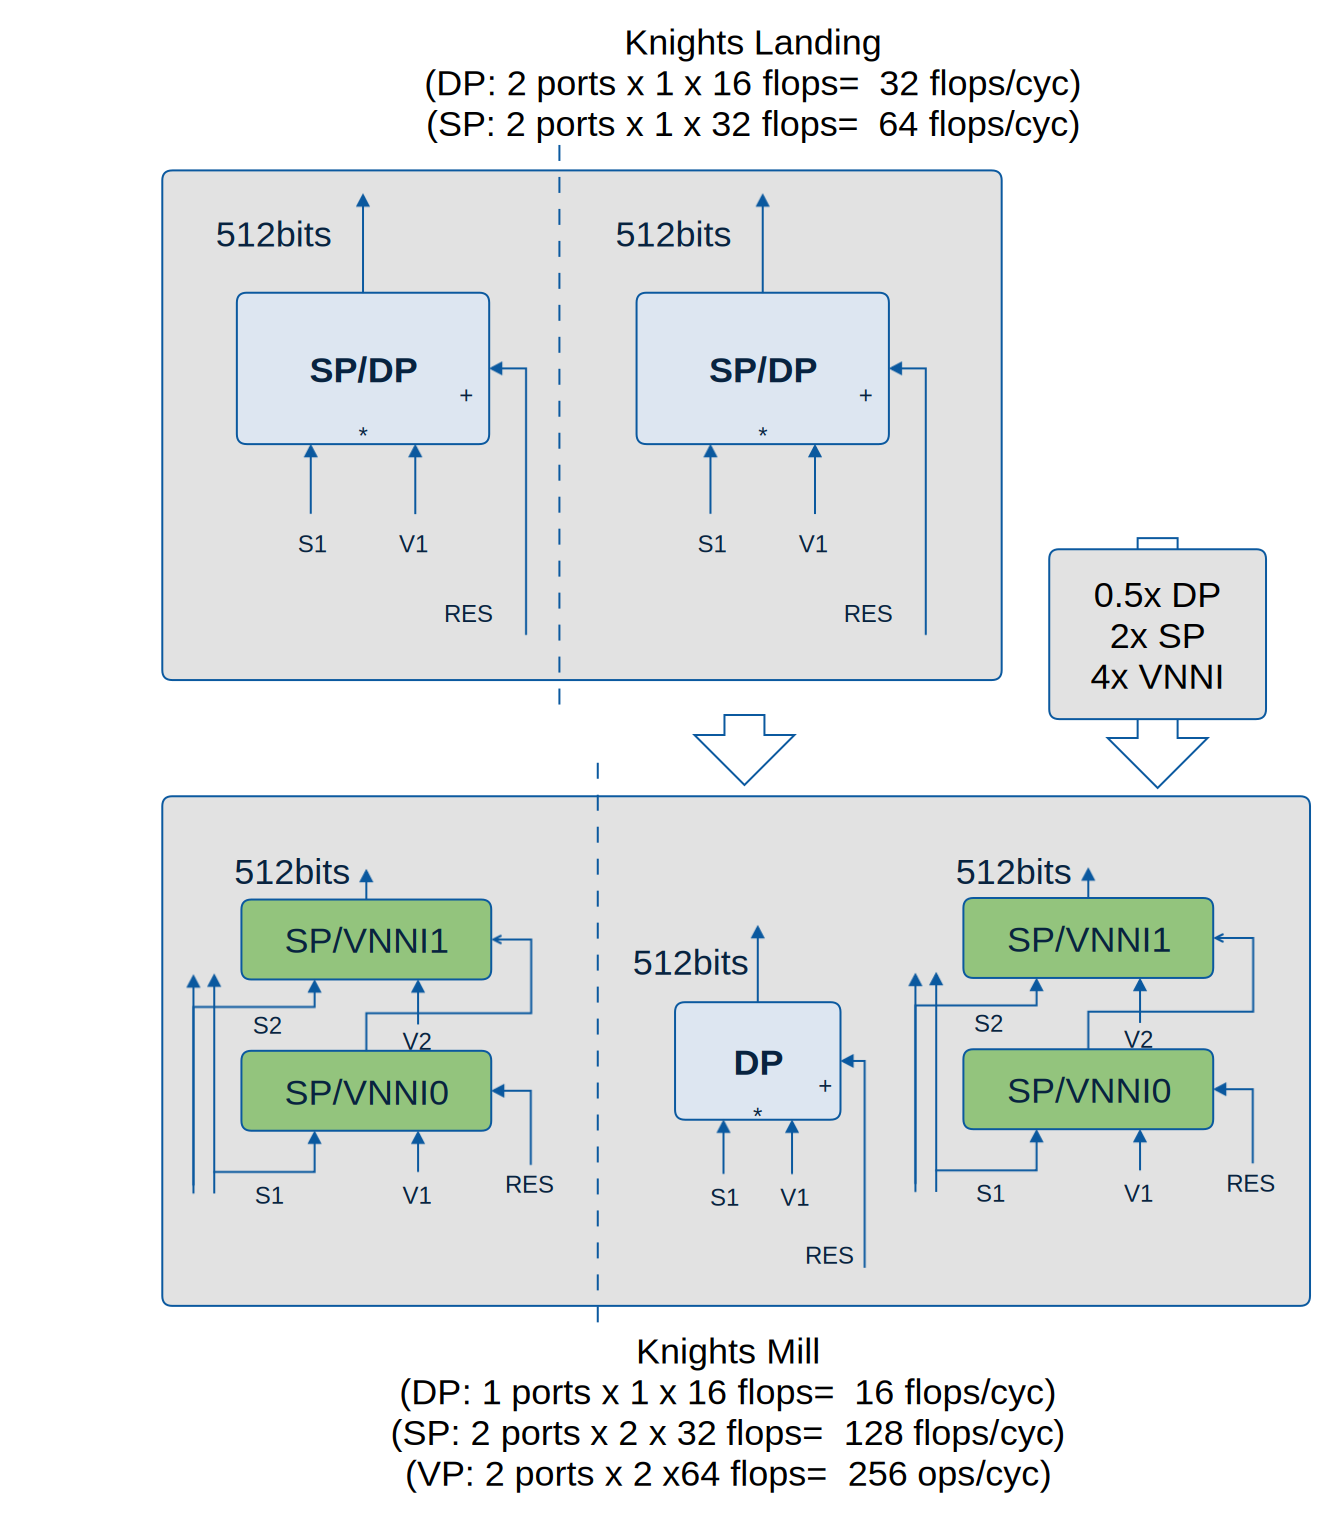
\includegraphics[width=.4\linewidth]{KNLvsKNM}
    \caption{\label{fig:knlvsknm}Comparison of KNL and KNM architecture\cJD{maybe too big for this little of for us relevant information?!; also have we referenced the original web/paper/etc?}}
\end{figure}

Intel Knight’s Landing (KNL) and Knight’s Mill (KNM) are the latest incarnations of a long line of architectures in the Intel’s accelerator family. Both processor consists of a large (64 and 72) number of processors cores, interconnected in a mesh interconnection (prior to KNL this was ring). Each core has a private L1 cache and a slice of the distributed L2 cache. Caches are kept coherent through directory-based MESIF protocol.
Both processors come with two types of external memory: MCDRAM (or, Hybrid Memory Cube, HMC) and Double-Data Rate-synchronous (DDR4) memory. Unique to the Xeon PHI processors is that the MCDRAM memory can be configured to one of two modes of operation: (1) it’s is either directly addressable in the global memory address space (memory-mapped), or (2) it acts as last-level cache before the DDR. The first configuration is called \texttt{flat} mode, and the second configuration is called \texttt{cache} mode, and a hybrid-mode mode\cite{heinecke_high_2016}) that combines properties from the the first two.
There are several policies governing where data is homed. A common high-performance configuration~\cite{gawande_scaling_2017}, which is also the one we used in our study, is the quadrant mode, meaning that the physical cores are divided into four logical parts, where each logical part is assigned two memory controllers; each logical group is treated as a unique Non-Uniform Memory-Access (NUMA) node, allowing the operating system to data-locality optimizations.
Table~\ref{table:HW} surveys and contrast the processors against each other, where the main differences are highlighted. The main architectural difference (Figure \ref{fig:knlvsknm}) – which is also the difference we seek to empirically quantify the impact of – is the Floating-Point Unit (FPU). In KNL, this unit features two 512-bit wide vector units (AVX), capable of executing 32 double-precision or 64 single-precision operations per cycle, totaling 2.6 and 13.8 TeraFLOP/s of double- and single-precision performance respectively across all 64 processing cores. In KNM, however, the FPU is redesigned to replace one of the 512-bit vector units with two Virtual Neural Network Instruction (VNNI) units; these units, although specializing in hybrid-precision FMA, can execute single-precision vector instructions, but have no support for double-precision compute. Thus, in total, the KNM can execute up-to 1.7 TeraFLOP of double-precision or 13.8 TeraFLOP of single-precision computations per second. In summary, the KNM has 2.59x more single-precision compute, while the KNL have 1.54x more double-precision compute.
While both the KNL and KNM are functionally and architectural similar, there are some note-worth differences. First, the operating frequency of the processor vary: the KNL operates at a frequency of 1.3 GHz (and up-to 1.5 GHz in Turbo mode), while KNM operates at 1.5 GHz (1.6 GHz turbo) -- KNM executes 15\% more cycles per second over KNM. Furthermore, although the cores of KNM and KNL are similar (except the FPU), the number of cores are different: KNL has 63 cores while KNM has 72 cores. Both processors are manufactured in 14 nm technology. Finally, the amount of on-chip last-level cache between the two processors is different, where KNM has a 4 MB advantage over KNL.
Finally, for verification reasons, we included a modern Intel Xeon processor in our evaluation. Although vastly different than the Xeon PHI systems, the Xeon general-purpose processor was used to cross-check metrics against, metrics such as: execution time and performance (Xeon PHI’s should perform better), frequency-scaling impact experiments (The Xeon has more frequency domains), and performance counters (the Xeon has far more performance counters).
Aside from the difference mentioned here (and highlighted in Table~\ref{table:HW}), the setup between the Xeon PHIs was \textit{identical}, including the same operating system, software stack, and solid state disk (mSSD SATA, 500 GB, Crucial).

\struc{add important notes on: linux kernel version and parameters, spector/meltdown patches, run levels, OS noise
from NFS, other users, special settings to pre-installed OS/gnu/linux tools, ...; since we removed the info from the table}

%Meanwhile, KNM has new instructions such as Quad Fused Multiply Add (QFMA),Variable precision instructions and Quad Virtual Neural Network Instruction (QVNNI). It is claimed by Intel that QFMA instructions enable 2x of the SP performance against KNL. Variable precision instructions help to get higher throughput in machine learning tasks. And QVNNI, the 16-bit INT operations are 4x faster than KNL's SP under the condition that Intel claims users can achieve “similar accuracy to single-precision.” with INT32 accumulated output.[see comment]
%[refer to slide https://indico.cern.ch/event/595059/contributions/2499304/attachments/1430242/2196659/Intel_and_ML_Talk_HansPabst.pdf]
%https://www.hpcwire.com/2017/06/22/knights-mill-gets-deep-learning-flops/
%One significant difference between Intel Xeon phi and Xeon is that Xeon phi have Multi-Channel DRAM (MCDRAM), which have a high bandwidth and relatively low capacity. There are several modes when using MCDRAM: cache mode, flat mode and hybrid mode.
%In cache mode, the MCDRAM will be performed as the last level cache. While in flat mode, MCDRAM will be used as memory. The hybrid mode is a mixture of the cache mode and flat mode.\cite{heinecke_high_2016}
%The mesh of Xeon phi can be operated in three different cluster modes: All2All mode, Quadrant mode and Sub-NUMA-Clustering(SNC4) mode.
%In All2All mode, no affinities are set. In Quadrant mode, the mesh will be divided into 4 logical parts and each memory controller will be mapped to one of four tag directories there belong to. For SNC4 mode, it is an extended version of the Quadrant mode, which exposes the four parts via NUMA domains to the OS.
%Nitin A. et al. in paper \cite{gawande_scaling_2017} discussed that which configuration should be chosen for a better performance. It is discussed that, cache mode + quadrant mode could be a better choice. Although AVX-512 instructions could benefit from flat mode, it need additional optimization to obtain the benefit.

\subsection{Benchmark Applications}\label{ssec:bm}

%\struc{small introduction sentence to this subsection and why it is relevant}

%\struc{introduce the ECP and postK mini-app projects, and why it is relevant for HPC and procurement}

%\struc{write short info about each application: what does it do, which science field it belongs to, what subproblem does the input data/parameter simulate, which category does it belong to (see riken study about code categories), byte2flop ratio if know from prev. publications}

The HPC community has developed many benchmarks representing real workloads or testing the
capabilities of a system, primarily for comparisons across architectures but also for system
procurement purposes.
The so-called Exascale Computing Project (ECP) proxy applications~\cite{noauthor_ecp_2018} and
RIKEN AICS' Fiber Miniapp Suite~\cite{riken_aics_fiber_2015}, which we will focus on for this study, are just
two examples representing the modern HPC workloads.
These benchmarks are designed to evaluate single-node and small-scale test installations,
and hence adequate for our study.


\subsubsection{ECP Proxy-Apps}\label{ssec:ecp}
The ECP benchmark suite (release 1.0) consists of twelve proxy applications primarily written in C (5x),
FORTRAN (3x), C++ (3x), and Python (1x).

\paragraph{Algebraic multi-grid (AMG)} solver of the \textit{hypre} library is a parallel solver
for unstructured grids~\cite{park_high-performance_2015} arising from fluid dynamics problems.
We choose \textit{problem~1} for our tests, which applies a 27-point stencil on a 3-D linear system.
%https://github.com/LLNL/AMG/blob/master/docs/amg.README: AMG is also memory-access bound, doing only
%about 1-2 computations per memory access, so memory-access speeds will also have
%a large impact on performance.

\paragraph{CANDLE (CNDL)} is a deep learning benchmark suite to tackle various problems in cancer
research~\cite{wozniak_candle/supervisor:_2018}.
We select benchmark 1 of pilot 1 (\textit{P1B1}), which builds an autoencoder from a sample of gene
expression data to improve the prediction of drug responses.

\paragraph{Co-designed Molecular Dynamics (CoMD)} serves as reference implementation for
ExMatEx~\cite{mohd-yusof_co-design_2013} to facilitate co-design for and evaluation of classical molecular
dynamics algorithms.
We are using the included strong-scaling example to calculate the inter-atomic potential for 256,000 atoms.
%https://www.lanl.gov/orgs/adtsc/publications/science_highlights_2013/docs/Pg88_89.pdf

\paragraph{LAGrangian High-Order Solver -- Laghos (LAGO)} computes compressible gas dynamics though
an unstructured high-order finite element method~\cite{dobrev_high-order_2012}. The input for our study is the
simulation of a 2-dimensional Sedov blast wave with default settings as documented for the
Laghos proxy-app.

\paragraph{MACSio (MxIO)} is a synthetic Multi-purpose, Application-Centric,
Scalable I/O proxy designed to closely mimic realistic I/O workloads of
HPC applications~\cite{dickson_replicating_2016}. Our input causes MACSio to write a total of \unit[433.8]{MB} to disk.

\paragraph{MiniAMR (MAMR)} is a adaptive mesh refinement proxy application of the Mantevo 
project~\cite{heroux_improving_2009} which applies a stencil computation on a 3-dimensional space,
in our case a sphere moving diagonally through the cubic medium.
%The cube is evenly distributed onto the processes, and adaptive meshing is performed for workload balancing.

\paragraph{MiniFE (MiFE)} is a reference implementation of a implicit finite elements 
solver~\cite{heroux_improving_2009} for scientific methods resulting in unstructured 3-dimensional grids.
For our study, we use 128$\times$128$\times$128 input dimensions for the grid.

\paragraph{MiniTri (MTri)} is able to apply different graph detection algorithms for a given graph,
such as community detection or dense subgraph detection~\cite{wolf_task-based_2015}.
As input for the triangle detection and approximation of the graph's largest clique, we downloaded
BCSSTK30 from the MatrixMarket~\cite{boisvert_matrix_1997}.

\paragraph{Nekbone (NekB)} is a proxy for the Nek5000 application~\cite{argonne_national_laboratory_nek5000_nodate}, and uses the conjugate
gradient method for solving the standard Poisson equation for computational fluid dynamics problems.
We enabled the multi-grid preconditioner, and for strong-scaling, see Section~\ref{ssec:metrics},
we fixed the elements per process and polynomial order to one number, respectively.

\paragraph{SW4lite (SW4L)} is a proxy for the computational kernels used in the seismic modelling
software, called SW4~\cite{petersson_users_2017}, and we use the \textit{pointsource} example, which calculates the wave
propagation emitted from a single point in a half-space.

\paragraph{SWFFT (FFT)} represents the compute kernel of the HACC cosmology application~\cite{habib_hacc:_2016}
for N-body simulations. The 3-D fast Fourier transformation of SWFFT emulates
one performance-critical part of HACC's Poisson solver. In our tests, we perform 32 repetitions on a
128$\times$128$\times$128 grid.

\paragraph{XSBench (XSBn)} is the proxy for a Monte Carlo calculations used by a neutron particle transport
simulator for a Hoogenboom-Martin nuclear reactor~\cite{tramm_xsbench_2014}. We simulate a \textit{large} reactor model
represented by a \textit{unionized} grid with $15\cdot10^6$ cross-section lookups per particle.


\subsubsection{RIKEN Mini-Apps}\label{ssec:postk}
In comparison to the modernized ECP proxy-apps, RIKEN's eight mini-apps are written in
FORTRAN (4x), C (2x), and a mix of FORTRAN/C/C++ (2x).

\paragraph{FrontFlow/blue (FFB)} uses the finite element method to solve the incompressible Navier-Stokes
equation for thermo-fluid analysis~\cite{guo_basic_2006}.
We simulate the 3-D cavity flow in a rectangular space discretized into 50$\times$50$\times$50 cubes.

\paragraph{Frontflow/violet Cartesian (FFVC)} falls into the same problem class as
FFB, however the difference is that FFVC uses the finite volume method (FVM)~\cite{ono_ffv-c_nodate}.
Here, we calculate the 3-D cavity flow in a 144$\times$144$\times$144 cuboid.

\paragraph{MODYLAS (MDYL)} makes use of the fast multipole method for long-range force evaluations in
molecular dynamics simulations~\cite{andoh_modylas:_2013}.
Our input is the \textit{wat222} example which distributes 156,240 atoms over a
16$\times$16$\times$16 cell domain.

\paragraph{many-variable Variational Monte Carlo (mVMC) method} implemented by this mini-app is used
to simulate quantum lattice models for studying the physics of condensed matter~\cite{misawa_mvmc--open-source_2018}.
We use mVMC's included strong-scaling test, but downsize it (1/3 lattice dimensions and 1/4 of samples). 

\paragraph{Nonhydrostatic ICosahedral Atmospheric Model (NICM)} is a proxy of NICAM, which
computes mesoscale convective cloud systems based on FVM for icosahedral grids~\cite{tomita_new_2004}.
We run Jablonowski's baroclinic wave test (\textit{gl05rl00z40pe10}), but reduce the
simulated days from~11~to~1.

\paragraph{Next-Gen Sequencing Analyzer (NGSA)} is a mini-app of a genome analyzer and a set of
alignment tools designed to facilitate cancer research by detecting genetic mutations in
human DNA~\cite{riken_csrp_grand_2013}.
For our experiments, we rely on pre-generated pseudo-genome data (\textit{ngsa-dummy}).

\paragraph{NTChem (NTCh)} implements a computational kernel of the NTChem software framework
for quantum chemistry calculations of molecular electronic structures, i.e., the solver for the
second-order M{\o}ller-Plesset perturbation theory~\cite{nakajima_ntchem:_2014}. We select the
H\textsubscript{2}O test case for our study.

\paragraph{Quantum ChromoDynamics (QCD)} mini-app solves the lattice QCD problem in a 4-D
lattice (3-D plus time), represented by a sparse coefficient matrix, to investigate the
interaction between quarks~\cite{boku_multi-block/multi-core_2012}. We evaluate QCD with the \textit{Class 2}
input for a $32^3 \times 32$ lattice discretization.


\subsubsection{Reference Benchmarks}\label{ssec:refbm}

Additionally, to these 20 applications, we will be using the compute intensive HPL~\cite{dongarra_linpack_1988} benchmark,
and HPCG~\cite{dongarra_new_2016} and stream (both memory intensive) to evaluate
the baseline of the investigated architectures. 

\paragraph{High Performance Linpack (HPL)} is solving a dense system of linear equations $Ax = b$
to demonstrate the double-precision compute capabilities of a (HPC)
system~\cite{strohmaier_top500_2018}. The problem size is 64,512.
% for a non-embarrassingly parallel problem and is used for system's placement in the TOP500
%list~\cite{hpl,top500}.
For both HPL and HPCG (see below), we employ highly tuned versions shipped with Intel's Parallel Studio
XE suite with appropriate inputs for our systems.

\paragraph{High Performance Conjugate Gradients (HPCG)} is applying a conjugate gradient solver
to a system of linear equation (sparse matrix $A$), with the intent to
demonstrate the system's memory subsystem and network limits. We choose 360$\times$360$\times$360 as
global problem dimensions for HPCG.

\paragraph{BabelStream (BABL)} is one of many available ``stream'' benchmarks supporting
evaluations of the memory subsystem for CPUs and accelerators~\cite{deakin_gpu-stream_2016}.
We will use~\unit[2]{GiB} and~\unit[14]{GiB} input vectors, see Section~\ref{ssec:eval_mem}
for details.

%
%
%
%There are small, simplified applications called proxy/mini applications in High Performance Computing (HPC). They allow application developers to share major features of their large applications while collaborators do not need to understand the complex code of original applications.
%
%Since the proxy can represent the most important features of the original applications, we use 23 HPC (proxy/mini) applications from various scientific domain, including 12 ECP Proxy applications and 8 Post-K Mini applications as our benchmark applications. We also used HPL, HPCG and STREAM as a comparison for analysis. Table \ref{table:APP} shows the list of benchmarks.
%
%\textbf{ECP Proxy Applications:} the ECP proxy app suite is created by ECP for representing the most important features (especially performance) of exascale applications.
%
%the Exascale Proxy Applications Project mainly focuses on improving the quality of proxies created by ECP and maximizing the benefit received from their use. To accomplish this goal, an ECP proxy app suite composed of proxies developed by ECP projects that represent the most important features (especially performance) of exascale applications will be created.
%\textbf{Post-K Mini applications (Fiber):} Fiber is a suite of miniapps that are maintained and developed at RIKEN Advanced Institute for Computational Science (RIKEN AICS).
%
%\cJD{this table is way to bloated, need a smaller with bench + science category + kernel classification (riken study) (+maybe byte2flop ratio if fits in 1 column)}
%\cJD{either full width and split left/right as now or single-column}
%\cJD{testing something: \ref{table:APP}}

We provide a compressed overview of the ECP and RIKEN's proxy applications in Table~\ref{table:APP}.
In this table, each application is categorized by its scientific domain, as well as the primary
workload/kernel classification, for which we use the classifiers employed by Hashimoto et al.~\cite{hashimoto_empirical_2017}.
%https://dl.acm.org/citation.cfm?id=3030217
Both, the scientific domain as well as the kernel classification will be important for our subsequent
analysis in Sections~\ref{sec:eval} and~\ref{sec:discuss}.
%
\begin{table}[tbp]
    \caption{\label{table:APP} Application Categorization and Compute Patterns; MACSio, HPL, HPCG, and BabelStream Benchmarks omitted\cJD{prof lang if space}}
    \centering
    \begin{tabular}{|l|l|l|}
        \hline \hC
        \tH{ECP}    & \tH{Scientific/Engineering Domain}    & \tH{Compute Pattern}    \\ \hline
        AMG         & Physics and Bioscience                & stencil       \\ \hline \rC
        CANDLE      & Bioscience                            & dense matrix  \\ \hline
        CoMD        & Material Science/Engineering          & N-body        \\ \hline  \rC
        Laghos      & Physics                               & \cJD{?}       \\ \hline
        %MACSio      & \textit{I/O benchmark}                & \textit{read/write}   \\ \hline
        miniAMR     & Geoscience/Earthscience               & stencil       \\ \hline \rC
        miniFE      & Physics                               & \cJD{?}       \\ \hline
        miniTRI     & Math/Computer Science                 & irregular     \\ \hline \rC
        Nekbone     & Math/Computer Science                 & \cJD{?}       \\ \hline
        SW4lite     & Geoscience/Earthscience               & \cJD{?}       \\ \hline \rC
        SWFFT       & Physics and Math/Computer Science\cJD{?}           & \cJD{?}  \\ \hline
        XSBench     & Physics                               & \cJD{?}       \\ \hline\hline \hC
        \tH{RIKEN}  & \tH{Scientific/Engineering Domain}    & \tH{Compute Pattern}   \\ \hline
        FFB         & Engineering (Mechanics, CFD)          & stencil       \\ \hline \rC
        FFVC        & Engineering (Mechanics, CFD)          & stencil       \\ \hline
        mVMC        & Physics                               & \cJD{?}       \\ \hline \rC
        NICAM       & Geoscience/Earthscience               & stencil       \\ \hline
        NGSA        & Bioscience                            & irregular     \\ \hline \rC
        MODYLAS     & Physics and Chemistry                 & N-body        \\ \hline
        NTChem      & Chemistry                             & dense matrix  \\ \hline \rC
        QCD         & Lattice QCD                           & stencil       \\ \hline
    \end{tabular}                                     
\end{table}

% 1.5 page

\section{Methodology}\label{sec:methods}
%
%\struc{small introduction sentence to this section}
In this section, we present our rigor benchmarking approach into investigating the characteristics of each architecture, and extracting the necessary information for our study.
%
% goal: 1.5 page
% no changes to any code (unless fixing bug)
% 2 similar architecture, executed lots of bench for flops/memory/power
% normalize results on #cores (avoid bad numa settings); change freq to 1.3GHz; etc -> to reduce obvious differences betw KNL/KNM
% xhost, intel, same compile
% run parameter sweep
%    #runs per app -> min/max/avg???
% strong scaling vs weak scaling
% tools/profileer/etc used ("exclusive" to intel SW stack + open-source)
% subsection on oddities of our config:
%    compiler/OS/kernel (w/ meltdown patch)
%    stupid mcdram behavior -> warm up ...
%    intel_pstate=disable for freq
%    fixed uncore freq.

\subsection{Benchmark Setup and Configuration Selection}\label{ssec:bmconf}
% \struc{assume BMs are well tuned}

Due to the fact that the benchmarks, listed in Section~\ref{ssec:bm}, are firstly realistic proxies of the
original applications~\cite{aaziz_methodology_2018} and secondly are used in the procurement process, we can confidently assume
that these benchmarks are well tuned and come with appropriate compiler options for a variety of compilers.
Hence, we refrain from both manual code optimization and alterations of the compiler options.
%
%\struc{how we compiled}
%
The only modifications we perform are:
\begin{itemize}
    \item Enabling interprocedural optimization (\texttt{-ipo}) and compilation for the highest instruction set available (\texttt{-xHost})\footnote{~Exceptions: (a) AMG compiled with \texttt{-xCORE-AVX2} to avoid arithmetic \\$~~~\,\quad$errors; (b) NGSA's BWA tool compiled with GNU gcc to avoid segfaults.},
    \item Patching a segmentation fault in MACSio\footnote{~After our reporting, the developers patched the upstream version.}, and
    \item Injecting our measurement source code, see Section~\ref{ssec:metrics}.
\end{itemize}
%
With respect to the measurement runs, we follow this five step approach for each benchmark:
\begin{enumerate}
    \item[0)] Install, patch, and compile the benchmark, see above, 
    \item Select appropriate inputs/parameters/seeds for execution,
    \item Determine ``best'' parallelism: \#processes and \#threads,
    \item Execute a \textit{performance}, a \textit{profiling}, and a \textit{frequency} run,
    \item Analyze the results (go to 0. if anomalies are detected).
\end{enumerate}
and we will further elaborate on those steps hereafter.

% \struc{strong scaling vs weak scaling, and mention exceptions to this rule (if any)}
%
%\struc{using recommended parameters or finding input/parameter thru trail/error to get targeted runtime of multi-seconds to avoid large run-to-run flutuations}
%
For the input selection we have to balance between multiple constraints and choose based on: Which
recommended inputs are listed by the benchmark developers?, How long does the benchmark run?\footnote{~Our
aim is~\unit[1]{sec}--\unit[10]{min} due to the large sample size we have to cover.} Does it occupy a
realistic amount of main memory (e.g., avoid cache-only executions)? Are the results repeatable
(randomness/seeds)? We optimize for the metrics reported by the benchmark (e.g., select the input
with the highest~\unit[]{Gflop/s} rate).
%
% \struc{explain parameter-sweep for num\_mpi and num\_omp, why, reason, how on all system,( and examples maybe)}
%
Furthermore, one of the most important considerations while selecting the right inputs is
\textit{strong-scaling}. We require strong-scaling properties of the benchmark for two reasons:
the results collected in Step~(2) need to be comparable, and even more importantly, the results
of Step (3) must be comparable between different architectures, since we may have to use different
numbers of MPI processes for KNL and KNL (and our BDW reference architecture) due to their difference
in core counts. The only exception is MiniAMR for which we are unable to find a strong-scaling
input configuration and instead optimized for the reported~\unit[]{Gflop/s} of the benchmark. Accordingly, we then choose
the same amount of MPI processes on our KNL and KNM compute nodes for MiniAMR.

In Step (2), we evaluate numerous combinations of MPI processes and OpenMP threads
%\cJD{any other threadin models?} -> candle uses omp-ish too, see
%https://simplecore.intel.com/nervana/wp-content/uploads/sites/53/2018/05/IntelAIDC18_Banu_Nagasundaram_Vikram_Saletore_5_24_Final.pdf
for each benchmark, including combinations which over-/undersubscribe the CPU cores, and test each
combination with three runs to minimize the potential for outliers due to system noise.
For all subsequent measurements, we select the number of processes and threads based on the ``best'' (w.r.t
time-to-solution of the solver) combination among these tested versions, see Table~\ref{table:rest} for details.
%\cJD{no specific intel' mpi tuning (except hpgc, babel) because initial test consistently resulted
%in worse time to solution when non-default options where used}
We are not applying specific tuning options to the Intel MPI library, except for using Intel's recommended
settings for HPCG with respect to thread affinity and MPI\_allreduce implementation.
The reason is that our pretests (with a subset of the benchmarks) with non-default parameters for
Intel MPI consistently resulted in longer time-to-solution.

%\struc{explain performance (10 runs select best) and profiling runs}
%
For Step (3), we run each benchmark ten times to identify the fastest time-to-solution for the
(compute) kernel of the benchmark. Additionally, for the profiling runs, we execute the benchmark
once for each of the profiling tools and/or metrics (in case the tool is used for multiple metrics),
see Section~\ref{ssec:metrics} for details. Finally, we perform frequency scaling experiments
for each benchmark, where we throttle the CPU frequency to all the available lower CPU states
below the maximum CPU frequency we use for the performance runs, and record the lowest kernel
time-to-solution among ten trials per frequency. The reason and results of the frequency scaling
test will be further explained in Section~\ref{ssec:eval_freq}.
One may argue for more than ten runs per benchmark to find the optimal time-to-solution, however,
given the prediction interval theory and our deterministic benchmarks executed on a single node,
it is unlikely to obtain a much faster run and we confirmed that the fastest~50\% of executions per
benchmark only vary by~3.9\% on average.
%
The collected metrics, see the following section, will be analyzed in Section~\ref{sec:eval} in detail.

%We measured on all applications by strong scaling. In each application, we changed multiple parameters such as the number of threads, the number of processes, the problem size, etc. and performed the experiment with configuration with the shortest execution time.
%
%We first read through the code and find the kernel part of these benchmarks. Then we added some code before and after the kernel section in order to identify the kernels for our measuring tools. 
%In order to change number of threads and processes, we used OpenMP and MPI. If these parameters changed, the execution time fluctuates. So we executed each program with any combinations
%number  of threads and processes. The variety of combinations depends on the architecture to be experimented.
%
%We compiled each application, fully specifying optimization options of Intel compiler.
%
%While avoiding cases that the execution time becomes too short to accurately collect results due to the measurement error, we chose parameters and input problems so that the execution would take much time.
%
% 今後出て来るMetricは特に断りのない限り、kernelを対象に計測したものとする(ここに書くよりもMetricで書くこと?)
%
%We sweep parameters using the combinations of factors of the number of CPU cores and find the fastest settings.
%
% \struc{explain frequency scaling test, and what it is useful for, maybe explain other methods we tried to get similar results}
%%% TODO: use this draft for eval_freq
%I can determine whether the application is computer-bound or memory-bound by changing frequency. In the case of compute-bound the speed changes in proportion to the frequency. In the case of memory-bound, the speed is kept.
%
% またそれぞれのMetricの実験は信頼性のため10回実験して、bestなものを採用した。
% And we profile the execution of each application 10 times and chose the result which has the shortest execution time.
%
% (Here is not true, I think should be:)
%We divide our tests into profile runs and performance runs. we do profile runs to get the amount of DP/SP operations that have nothing to do with the time. During performance runs, we run all the applications for at least 10 times and take the best one in order to get rid of the effect of the randomness or other unexpected problem.
% (done)


\subsection{Metrics and Measurement Tools}\label{ssec:metrics}
%
%\struc{all metrics hereafter are based on the extracted kernel unless otherwise stated}
%
% \struc{small introduction sentence to this subsection and why it is relevant}
%This section introduces the metrics we measured and the reason why we measured them.
%
To study and analyze the floating point requirements by applications, it is not only important to
evaluate an established metric (floating point operations per second), but also other metrics,
such as memory throughput, cache utilization, or speedup with increased CPU frequency.
%
The detailed list of metrics (and derived metrics) and the methodology and tools we use to
collect these metrics will be explained hereafter.

%\struc{identify solver/kernel/core of app and inject code for vtune/timeing/pcm/etc.}
%\cJD{need a small pseudo code showing the extraction of the kernels}
One observation is that the amount of time spent on initializing and post processing within
each proxy application can be relatively high (e.g., HPCG spends only~11\% and~30\% of its
time in the solver part on BDW and Phi, respectively) and is usually not consistent with the real workloads, e.g., one can
reduce the epochs for performance evaluation purposes in CANDLE but not the input data
pre-processing to execute those epochs. These mismatches in kernel-to-[pre$|$post]processing ratio
requires us to extract all metrics only for the (computational) kernel of the benchmark.
Hence, we identify and inject profiling instructions around the kernels to start or pause the
collection of raw metric data by the analysis tools. This code injection is exemplified in
PseudoCode~\ref{code:inj}. Therefore, unless otherwise stated in this Section or subsequent sections,
all presented data will be based exclusively on the kernel portion of each benchmark.
%
\begin{algorithm}[tbp]
    \label{code:inj}
    \SetKwProg{Fn}{Function}{ is}{end}
    \#define START\_ASSAY \{measure time; toggle on [PCM $|$ SDE $|$ VTune]\} \;
    \#define STOP\_ASSAY \{measure time; toggle off [PCM $|$ SDE $|$ VTune]\} \;
    \Fn{main}{
        STOP\_ASSAY\;
        {\color{gray}Initialize benchmark}\;
        \ForEach{{\color{gray} solver loop}}{
            START\_ASSAY\;
            {\color{gray}Call benchmark solver/kernel}\;
            STOP\_ASSAY\;
            {\color{gray}Post-processing}\;
        }
        {\color{gray}Verify benchmark result}\;
        START\_ASSAY\;
    }
    \caption{Injecting analysis instructions}
%    \vspace{-0.5em}
\end{algorithm}

%\struc{what does each tool have in terms of capabilities, how is it applied to the benchmarks,
%anything we had to fix, patch, do to the OS/kernel/benchmark to use tool XYZ}
%
For tool stability reason, attention to detail/accuracy, and overlap with our needs, we settle
on the use of the MPI API for runtime measurements, alongside with Intel's Processor Counter
Monitor (PCM)~\cite{willhalm_intel_2017}, Intel's Software Development Emulator (SDE)~\cite{raman_calculating_2015}, and Intel's VTune
Amplifier~\cite{sobhee_intel_2018}\footnote{~To avoid persistent compute node crashes, we had to use disable VTune's
\\$~~~\,\quad$build-in sampling driver and instead rely on Linux' perf tool.}.
Furthermore, as auxiliary tools we rely on RRZE's Likwid~\cite{treibig_likwid:_2010} for frequency
scaling\footnote{~Our Linux kernel version required us to disable
the default Intel P-State\\$~~~\,\quad$driver to have full access to the fine-grained frequency scaling.} and
LLNL's msr-safe~\cite{walker_best_2016} for allowing access to CPU model-specific registers.
An overview of (raw) metrics which we extract with these tools for the benchmarks, listed in
Section~\ref{ssec:bm}, is shown in Table~\ref{tb:Mtools}. Furthermore, derived metrics, such
as~\unit[]{Gflop/s}, will be explained on-demand in Section~\ref{sec:eval}.
%
\begin{table}[tp]
    \vspace{-0.5em}
    \centering\scriptsize
    \caption{\label{tb:Mtools}Summary of metrics and method/tool to collect these metrics}
    \begin{tabular}{|l|l|}
        \hline \hC
        \multicolumn{1}{c}{\textcolor{white}{Raw Metric}}   & \multicolumn{1}{c}{\textcolor{white}{Method/Tools}}   \\\hline
        Runtime [\unit[]{s}]                & MPI\_Wtime()                      \\\hline \rC
        \#\{FP / integer operations\}       & SDE                               \\\hline
        \#\{Branches operations\}           & SDE                               \\\hline \rC
        Memory throughput [\unit[]{B/s}]    & PCM (pcm-memory.x)                \\\hline
        \#\{L2/LLC cache hits/misses\}      & PCM (pcm.x)                       \\\hline \rC
        Consumed Power [\unit[]{Watt}]      & PCM (pcm-power.x)                 \\\hline
        SIMD instructions per cycle         & perf + VTune (`hpc-performance')  \\\hline \rC
        Memory/Back-end boundedness         & perf + VTune (`memory-access')    \\\hline
    \end{tabular}
    \vspace{-0.5em}
\end{table}

%
% \struc{which metrics are we collecting, how is each collected, and/or derived from other metrics, and
% most importantly: why do we care about this metric; add formulae if necessary}
%
%If you experiment with different precision, the data size will be different. We measure the memory size to see how much data is secured. Also we measure bandwidth and stall to see if data were actually used. We measure the Last Level Cache (LLC) to evaluate the performance of Metric on memory access.
%By showing the result of each metric together with the ratio of FP64 and FP32, it becomes possible to think about the meaning when the precision is changed. \cJD{we arent changing anything... stay on topic}
%
% 精度が異なることで、データサイズが変わってくる。どれだけデータが確保されたを示すのがmemory size。それが実際に使用されるかをみるのが、bandwidth、stall。
% llcは、その性能の理由を判断するのに必要な指標となる。
% 各メトリックスを、FP64とFP32の比率と共にしめすことで、精度を変更した場合にどれだけ意味を持つか、考えられるようになる。
% We measured power l,m 
%
%\subsection{Measuring tools}\label{ssec:tools}
%
%\struc{small introduction sentence to this subsection and why it is relevant}
% Tsuji wrote
% 何を用いて測定したかを示すことが「なぜ」重要かを示す
%   - To clarify the characteristic (e.g. assumptions, strengths, weaknesses) of the tools
%   - To clarify the purpose of the measurements
%   - To clarify how to reproduce the results
%
%Showing the tools of how we get the benchmark results are important in several aspects.
%One is to understand the characteristic of the tools. Some tools can put critical assumptions on application
%or have strengths/weakness for getting the metrics.
%Another is to reproduce the results.
%In this subsection, we will show the used tools and explain the main characteristics.
%
%
%To measure the power we used Intel Performance Counter Monitor (Intel-PCM).
%Intel-PCM is an API and a set of tools to monitor performance and energy metrics.
%We collected the energy (Joule) each 100 ms during the application is running, and averaged the
%total to compute the power (Joule per second).
% https://github.com/opcm/pcm
% https://software.intel.com/en-us/articles/intel-performance-counter-monitor
% Do we modified the original code? (Tsuji)
%
%% not relevant
%To measure the memory size we used Heaptrack.
%Heaptrack can trace all memory allocations and annotate these events with stack traces.
%We collected the peak memory consumption of the application and regarded it as the memory size of the
%application.
%% https://github.com/KDE/heaptrack
%
%Intel-PCM is used also for measuring memory bandwidth.
%Intel-PCM includes a binary called \texttt{pcm-memory.x}, it monitors memory bandwidth per-channel
%and per-DRAM DIMM rank.
%For Xeon-Phi architectures (KNL and NKM), we measured the MCDRAM bandwidth.
% Ask Matsumura is this correct
%
%To measure the number of pipeline stalls we used Intel VTune Amplifier (VTune).
%Using this tools we can collect the number of cycles issued no-op due to stalls.
% https://software.intel.com/en-us/vtune
% Ask Haoyu (Tsuji)
%
%To measure the number of LLC hits and misses we used Linux Performance Tools (Perf).
%The collected events in \texttt{perf stat} command for Xeon is ``r04D1'' and ``r20D1''.
% \cJD{WAY TO DETAILED and untrue (in the end we use intel pcm for it)}
%For Xeon-Phi it is ``uncore\_edc\_uclk\_0/period=0x0, inv=0x0, edge=0x0, event=0x0, umask=0x$N$, thresh=0x'',
%where $N = 1,2,4,8$.
%
%To measure the running time including initialization and finalization we used \texttt{date} command.
%And the time of solver, we inserted gettimeofday functions in the appropriate place in the code.\cJD{UNTRUE: we use MPI-wtime}
%
%To measure FLOPS/s we used Intel Software Development Emulator (Intel-SDE).
%Using Intel-SDE we collected the number of operations of double precision floating points, single precision floating points,
%and integer, including vector instructions.
%Dividing the number of operations with the running time inside of the solver, we could obtain the
%FLOPS/s for double precision and single precision.
%
%\struc{did we use other similar tools which we abandoned due to lack of accuracy, functionality, or stability, etc?}
%
%Valgrind was first used for measuring memory size, however due to lack of accuracy we moved to Heaptrack.
% http://valgrind.org
%
%Table \ref{tb:Mtools} shows the summary of the metrics and its corresponding tool.
%
%\begin{table}
%    \centering
%    \caption{\label{tb:Mtools}Summary of Measuring Tools}
%    \begin{tabular}{|c|c|c|}
%        \hline
%        Metrics & Tools\\
%        \hline
%        Power & Intel-PCM (201710)\\
%        \hline
%        Memory size & Heaptrack (v1.1.0)\\
%        \hline
%        Bandwidth & Intel-PCM (201710)\\
%        \hline
%        Number of stalls & VTune (2018.1.038)\\
%        \hline
%        Number of LLC hits/misses & Perf (3.10.0-693.17.1.el7.x86\_64.debug)\\
%        \hline
%        FLOPS/s & date command \& Intel-SDE\\
%        \hline
%    \end{tabular}
%\end{table}
%
% POWER: 身元不明。アターさんに聞く。
% MEMORY SIZE: HEAPTRACKを使用。
% BANDWIDTH: INTEL-PCMを使用。
% STALL: VTUNEを使用。オプションはスクリプトを参照。
% LLC: PERFを使用。
% FLOPS: timeコマンドで測った実行時間と、Intel SDEを使用。timeコマンドでは5回測ったうちの最短時間を使用。
% PCM、SDEの測定では、プログラムのカーネル部分の実行のみ対して行うようにしている。
% https://gitlab.m.gsic.titech.ac.jp/precision_experiments/mtmr/blob/master/ave_core.sh
% 1.5 page

\section{Evaluation}\label{sec:eval}
%
%\struc{small introduction sentence to this section}
The following subsections will primarily focus on visualizing and analyzing the key metrics we collected for each proxy- and mini-app,
such as \unit[]{Gflop/s}. The significance of our findings with respect to future software, CPU, and HPC system design will then
be evaluated in the next Section~\ref{sec:discuss}.
High or low \unit[]{operations/s}, see Section~\ref{ssec:eval_ops} and~\ref{ssec:eval_flops}, or \unit[]{byte/s}, see
Section~\ref{ssec:eval_mem}, by itself is not a good indication about the system's bottlenecks.
Especially, when reasoning about FPU requirements, we also have to understand the applications' compute-boundedness, which
we evaluate in Section~\ref{ssec:eval_freq}.

\struc{which metrics are we collecting, how is each collected, and/or derived from other metrics, and
most importantly: why do we care about this metric; add formulae if necessary}
%\struc{need at least: FP ratio, Int, freq scaling, memory BW, ...TBA}
%\cJD{have to analzye the run2run variation among the 10 speed runs} done that
%

% goal: 2.5 -- 3 pages
% language (report) + program desciption + (Minami-san classication M1-M6 or so for apps)
% run time overall (can measure but not strickly needed)
% time in solver
% abs numbers / percentage instructions
% performance in (sp/dp) gflop/s
% total #flops (part of 2. above)
% memory usage (peak mem util ; memory throughput; info from vtune?? for L1/L2/L3?) -> try carefully vtune
% !! fix uncore to max.
% !! KNL+KNM keep at max freq. (perf govenour + max fequ)
% resource stall counter (abs/percentage) -> vtune
% LLC hit/miss rate (also +L2 rates if in mcdram in cache; skip flat mode)
% fp64/fp32/int/(branch?)/(unconditional memory ops; -> LOAD/STORE) instructions -> get load/store from SDE (ask artur for details)
% power usage (use pcm-power and report per kernel number)
% memory-boundness, multitude of tests based on, and list all:
%  - educated guess + flops/to/bytes
%  - roof line (!skip)
%  - stalled instructions (artur: diff from resource stall counter)
%  - frequ. scaling -> least important item (skip if not needed)
%  - mcdram? vs ddr? (skip flat mode but report that we tried -> faster memory -> faster exec?)
%  - traffic betw. LLC and RAM (pcm-mem and CAREFUL about broken numbers on socket 1 on kiev)
%  (-- how much does each of these contribute to the ground-truth???)
% normalized based on number of core or absolute numbers, dep. on context/what to show
% ** create all graphs and check for the **anomalies**
%
% => all 3 systems (find kiev w/ right pcm results)
%
% put uninteresting stuff into TechReport
%
%% BM list
%
%  - memory foot print (ignore KNM because heaptrack broken -> but use lyon numbers to extrapolate)
%  - running scripts: jens has all
%  - scipts for  analysin g results : matsumura
%  - script for figure creating : matsumura
%  - master script: jens
%  - FORCED blackout aug! ->careful when to run
%  - solo on system (init 3?); any OS variance? SAME kernel! -> avoid the one with gnome (maybe lyon3+mill1+kiev5) -> maybe 3 ssd or ask nomura what best to isolate node (init 3 plus network stack maybe)
%  - take best time and recalculate mem throughput / power reported based on best time and not based on time in the run of pcm (if vastly different)
%
%matsumura: memory used on ngsa? heaptrack -> broken?
%matsumura: what is "copy of ..." sheets? flat or cache?
%yashima: KNL numbers updated for SW4lite: forgot to update colors or no yet updated?
%artur: powsample: reports processor or cpu+mem? we see 234W in one app on KNL whihc is above TDP (230W)
%jens: pcm-pwer: main result is cpu or node??? -> hamid: everything on the package
%jens: compare pcm-pwer vs powsameple for sw4lite
%artur: how can you have higher than TDP power? esp if BM/powersample reports power over time (avg?) and has like sw4lite a "big" init phase
%haoyu+yashima: compile CoMD/Sw4Lite with -mtune=core-avx2 instead of -xHost (to check if code has unvectorized instructions -> artur's theory)
%artur: original modylas problem: how to get instruction mix? to test this theory? which counters?
%hayou: perf defined as image per sec (instead of gflops or so)
%everyone: check jens's config skript for input data set? cross check -> want to run same everyone
%everyone: check analysis scripts together


\subsection{Integer vs. Single-Precision FP vs. Double-Precision FP}\label{ssec:eval_ops}
%
\begin{figure}[tbp]
    \centering
    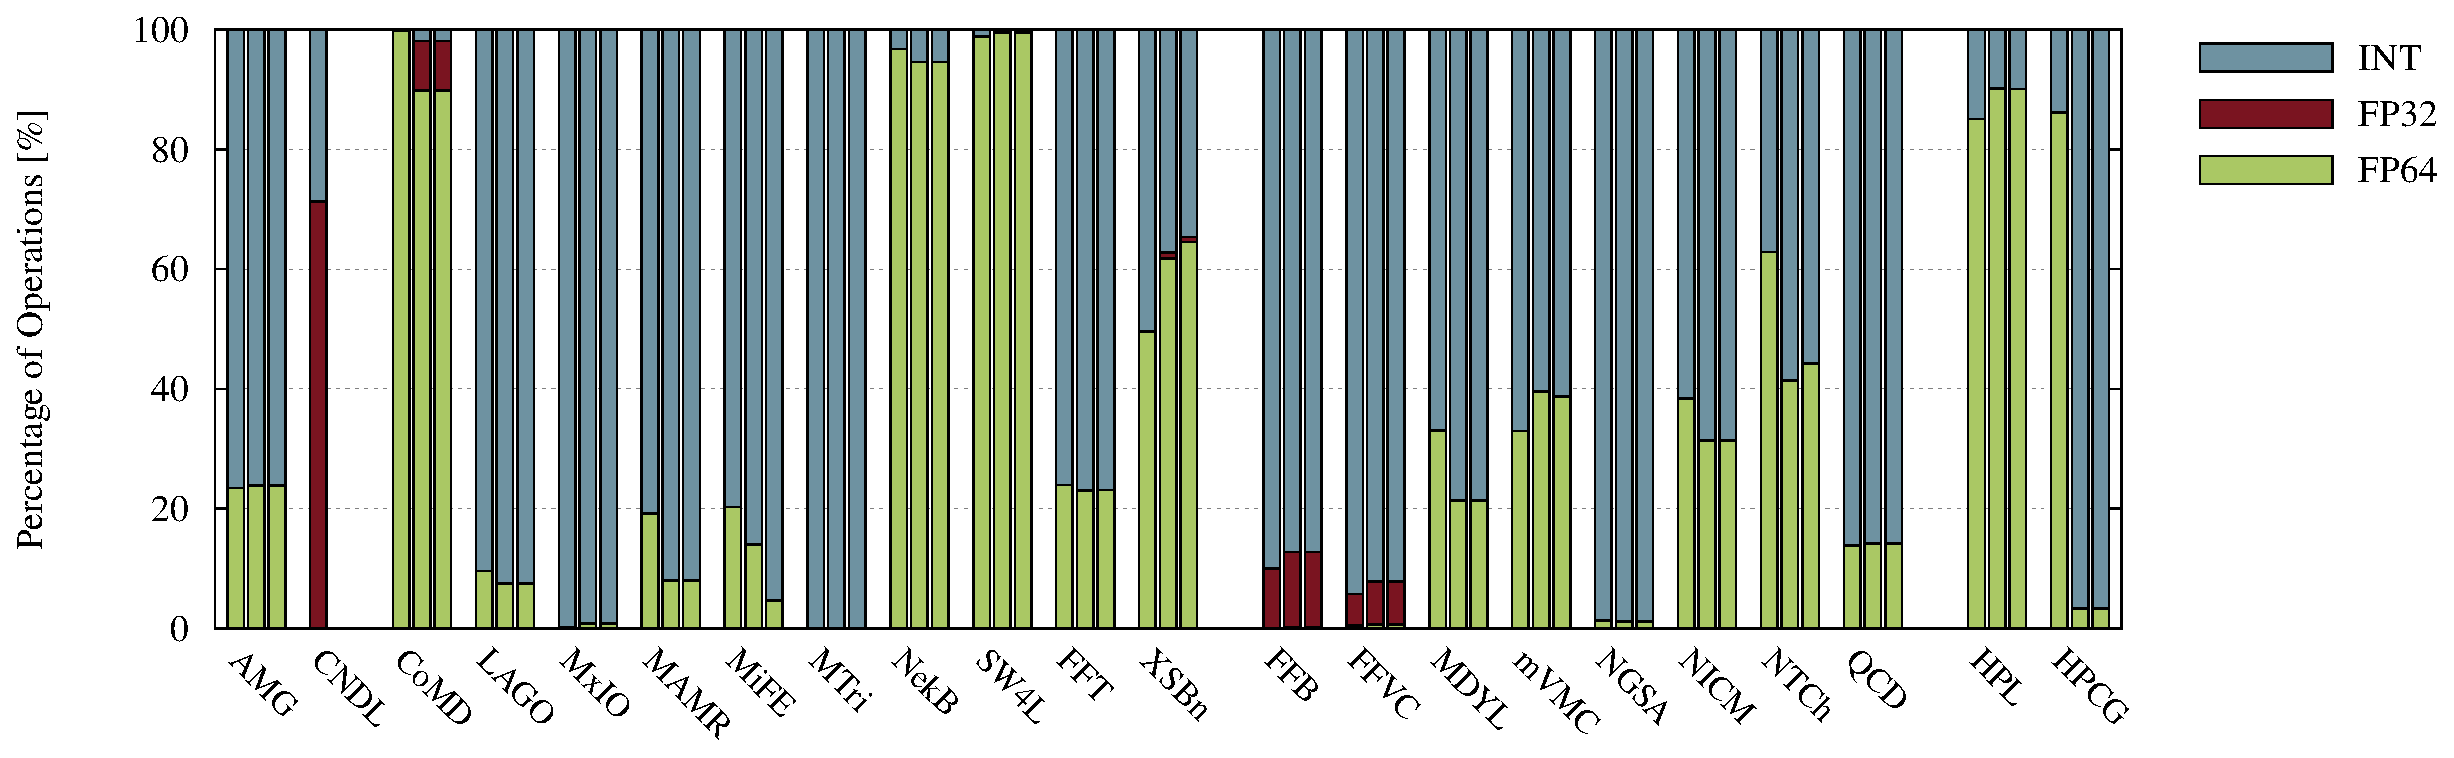
\includegraphics[width=\linewidth]{alu-fpu-ops}
    \caption{\label{fig:totalops} Ratio of Integer vs. single-precision FP vs. double-precision FP per proxy-app as counted by Intel's SDE; Per application: \textbf{Left bar = BDW, middle bar = KNL, right bar = KNM}; Missing bars for CANDLE due to SDE crashes on Xeon Phi; Proxy-app abbreviations acc. to Section~\ref{ssec:bm}}
\end{figure}
%
%\cJD{discuss the problem with int over-represented because of sde counting method}
The breakdown of total number of integer and single/double-precision FP operations, as depicted in Figure~\ref{fig:totalops},
shows two rather unexpected trends. First, the numbers of proxy-apps relying on 32-bit FP instructions is with four out of 22
surprisingly low, and furthermore, only one of them utilizes both 32-bit and 64-bit FP instructions.
Minor variances in integer to FP ratio between the architecture can likely be explained by the difference in
AVX vector length, quality of compiler optimization for each CPU, and execution/parallelization approach.
The second unexpected trend is the imbalance of integer to FP operations, i.e., 16 of 22 applications issue at least 50\%
integer operations. However, one has to keep in mind that Intel SDE output includes AVX vector instructions for integers, where
the granularity can be as low as 1-bit per operand (cf. 4 or \unit[8]{byte} per FP operand). Hence, the total integer operations
count might be slightly inflated.
Lastly, the results for HPCG show a big discrepancy between BDW and KNL/KNM. While the total FP operations count is similar,
the binary for KNL/KNM issues far more integer operations, see Table~\ref{table:rest} for details, and we are unaware of the reason.

\subsection{Floating-Point Op/s and Time-to-Solution}\label{ssec:eval_flops}
%
\begin{figure}[tbp]
    \centering
    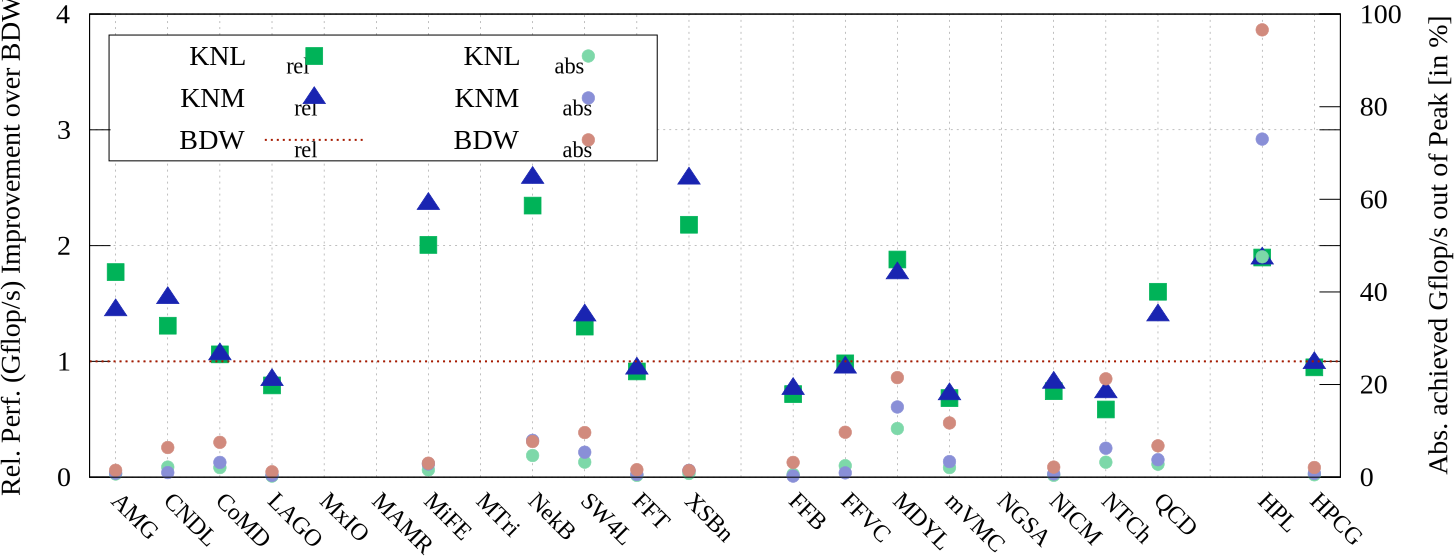
\includegraphics[width=\linewidth]{flops-rel}
    \caption{\label{fig:flops} Relative floating-point performance (FP32 and FP64 \unit[]{Gflop/s} accumulated) of KNL/KNM in comparison to dual-socket Broadwell-EP (see \textit{KEY}\textbf{\textsubscript{rel}}, left y-axis) and Absolute achieved \unit[]{Gflop/s} w.r.t dominant FP operations (cf. Fig.~\ref{fig:totalops}) in comparison to theoretical peak performance listed in Tab.~\ref{table:HW} (see \textit{KEY}\textbf{\textsubscript{abs}}, right y-axis); Due to missing SDE data for CANDLE, we assume the total number of FP operations is equivalent to BDW and divide by CANDLE's time-to-solution; Filtered proxy-apps with negligible FP operations: MxIO, MTri, and NGSA; Filtered out MiniAMR because of the strong-scaling issue described in Section~\ref{ssec:bmconf}; Proxy-app abbreviations acc. to Section~\ref{ssec:bm}}
\end{figure}
\begin{figure}[tbp]
    \centering
    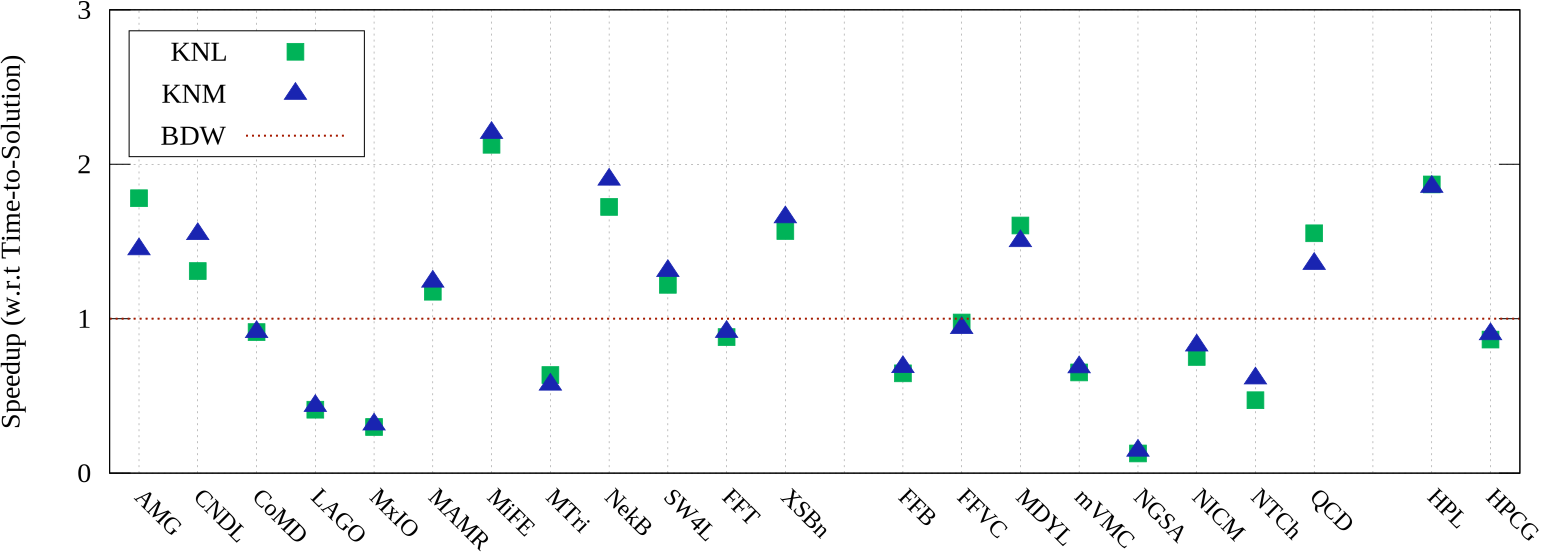
\includegraphics[width=\linewidth]{t2s-rel}
    \caption{\label{fig:t2s-knl-vs-knm} Speedup of KNM over KNL as baseline. MiniAMR included since the input is the same for both Phi\cJD{why call out MiniAMR?}; Proxy-app abbreviations acc. to Section~\ref{ssec:bm}}
\end{figure}
%
Figure~\ref{fig:flops} shows the relative performance improvement of KNL/KNM over BDW dual socket and the absolute achieved GFLOPS on each processor. It is important to note that all proxy/miniapps, with the exception of HPL, have less than 21.5\% (BDW), 10.5\% (KNL), and 15.1\% (KNM) FP efficiency. Given that the proxy/miniapps are largely optimized, and still achieve this low efficiency, implies the limited 
\cJD{Figure~\ref{fig:t2s-knl-vs-knm} mostly get faster from slightly higher freq it seem, ecept candle which benefits from VNNI and
NTCh seem to be a strange outlier, some memory-bound apps (AMG, HPCG, MTri) get slower, maybe because of the difference in peak bw
we see in figure~\ref{fig:memthru} and the increased core count competing for bandwidth}
\cJD{hence, looking at fp 64 or 32 in the context of mini-apps is almost stupid...}

\subsection{Memory Throughput of (MC-)DRAM}\label{ssec:eval_mem}
%
\begin{figure}[tbp]
    \centering
    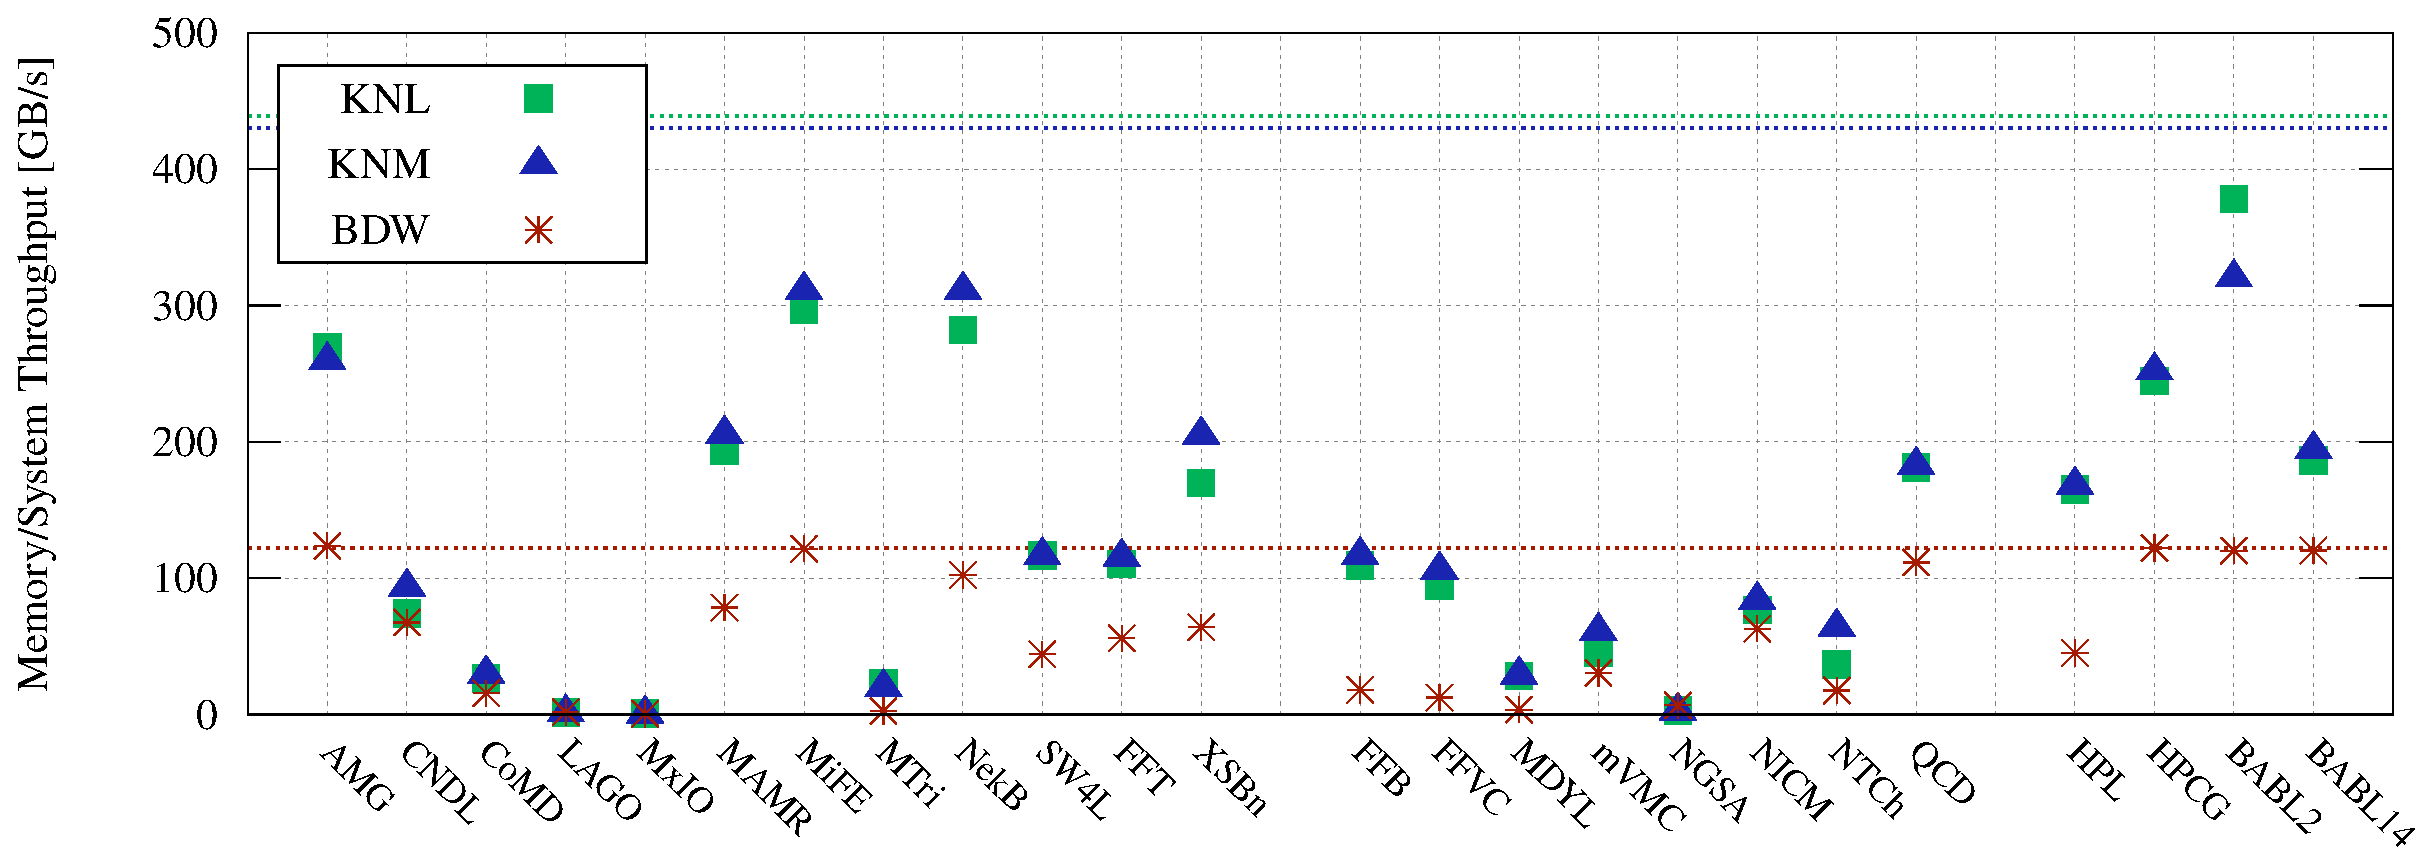
\includegraphics[width=\linewidth]{mem-throughput}
    \caption{\label{fig:memthru} Memory throughput (only DRAM for BDW, DRAM+MCDRAM for Phi) per proxy-app; Dotted lines indicate Triad stream bandwidth (flat mode, cf. Tab.~\ref{table:HW}); BabelStream for \unit[2]{GiB} (BABL2) and \unit[14]{GiB} (BABL14) vector length added (measured in cache mode); Proxy-app labels acc. to Section~\ref{ssec:bm}}
\end{figure}
%
For the memory throughput measurements, shown in Figure~\ref{fig:memthru}, we use Intel's PCM tool to analyze DRAM and MCDRAM throughput.
Our measurements with BabelStream are included as well to demonstrate the maximum achievable bandwidth, see horizontal lines for MCDRAM
in \textit{flat mode}), which is lower when the MCDRAM is used in \textit{cache mode}.
We still achieve 86\% on KNL and 75\% on KNM when the vectors fit into MCDRAM, but drop to slightly
higher than DRAM throughput (due to minor prefetching benefits) when the vectors do not fit (see BABL14 for \unit[14]{GB} vectors).
This throughput advantage of the MCDRAM translates into a performance boost for six proxy-apps (AMG, MAMR, MiFE, NekB, XSBn, and QCD)
which heavily utilize the available bandwidth, see Figure~\ref{fig:memthru}, and which are memory-bound on our reference system
This can easily be verified when comparing the time-to-solution for the kernels listed in Table~\ref{table:rest}.
Only HPCG cannot benefit from the higher bandwidth and, despite showing $\approx$2x throughput, the runtime drops by more than 10\%,
indicating a memory-latency issue of HPCG on KNL/KNM, which was one of the design goals for the benchmark~\cite{dongarra_new_2016}.
%
%\begin{figure}[tbp]
%    \centering
%    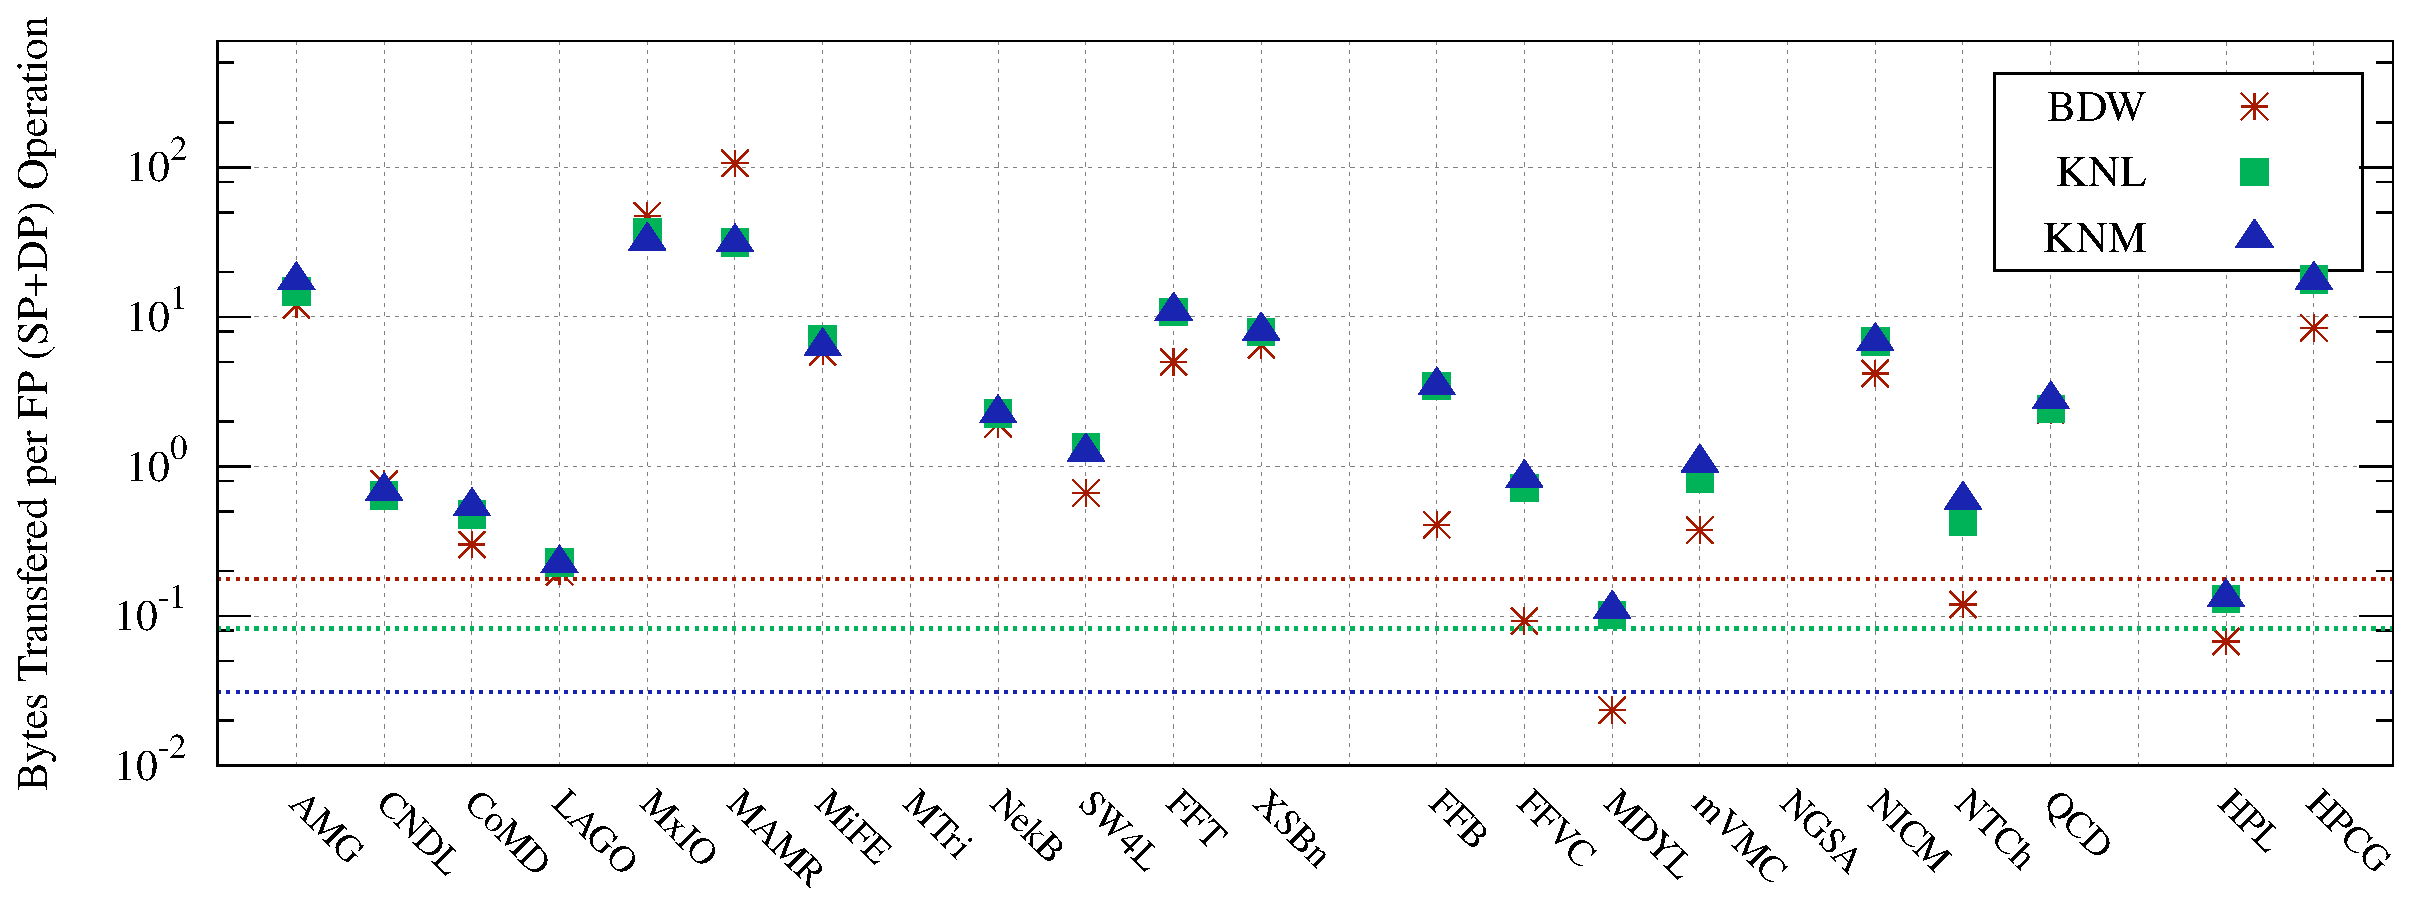
\includegraphics[width=\linewidth]{bpf-ratio}
%    \caption{\label{fig:bpfratio} \cJD{do we have space for bytes-per-flop?}}
%\end{figure}

\subsection{Frequency Scaling to Identify Compute-Boundedness}\label{ssec:eval_freq}
%
\begin{figure}[tbp]
    \centering
    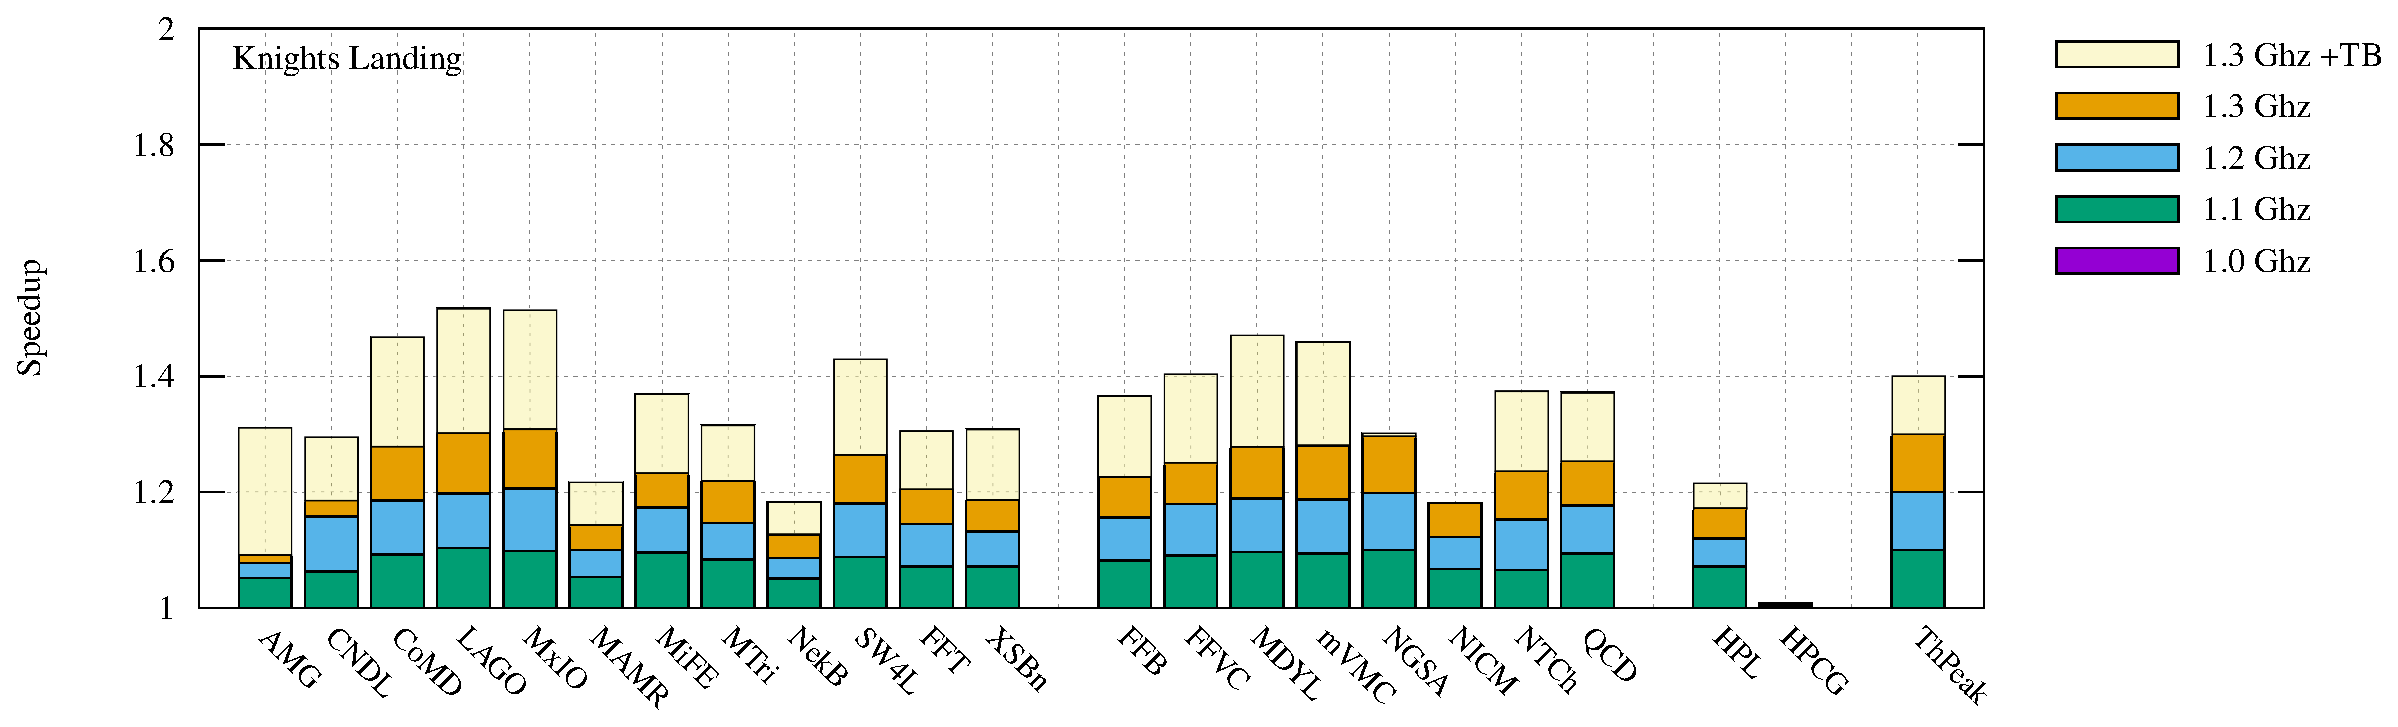
\includegraphics[width=\linewidth]{knl-freq}
    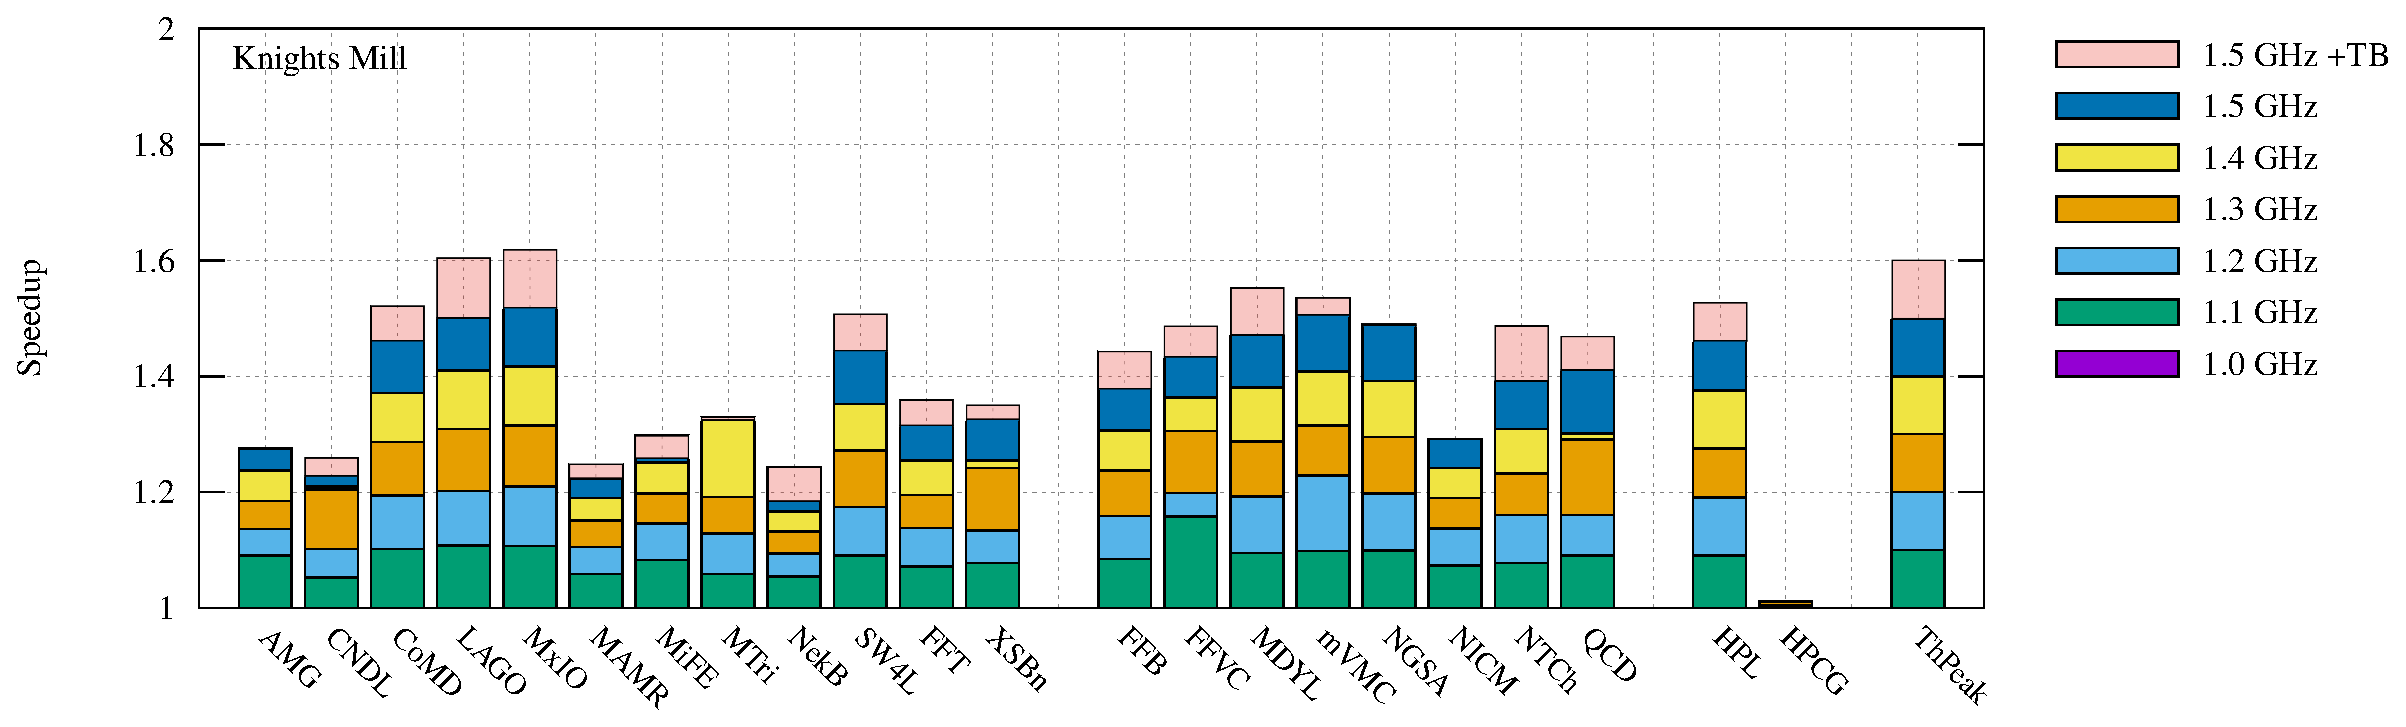
\includegraphics[width=\linewidth]{knm-freq}
    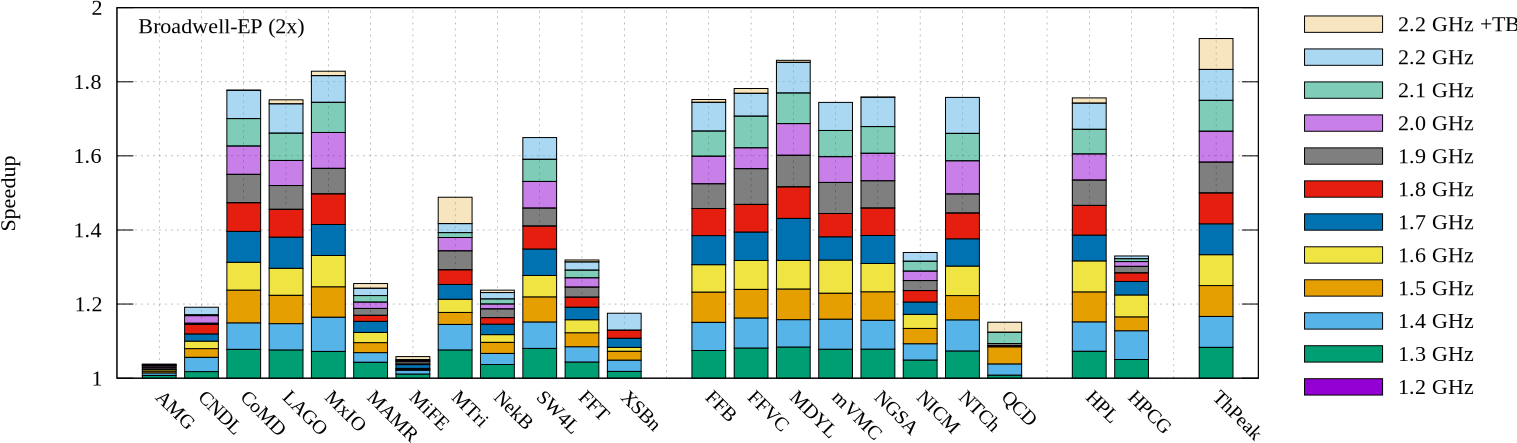
\includegraphics[width=\linewidth]{bdw-freq}
    \caption{\label{fig:freq} Speedup obtained through increased CPU frequency (w.r.t baseline frequency of \unit[1.0]{Ghz} on KNL/KNM and \unit[1.2]{Ghz} on BDW); \textbf{Top plot: KNL, middle plot: KNL, bottom plot: BDW}; Theoretical peak (ThPeak): furthest right bar; Labels/abbreviations of proxy-apps according to Section~\ref{ssec:bm} and 'TB' = Turbo Boost is assumed to be \unit[100]{Mhz} across all cores}
\end{figure}

For this test, we disable turbo boost and throttle core frequency, but keep uncore at maximum frequency which would otherwise negatively
affect the memory subsystem, to identify each application's dependency on ALU/FPU performance. The shown speedup (w.r.t time-to-solution) in Figure~\ref{fig:freq}
of each proxy-app is relative to the lowest CPU frequency on each architecture, and we include our \textit{performance} results
(cf. Section~\ref{ssec:bmconf}) with max.~frequency plus enabled turbo boost.

%\cJD{ecp on bdw mostly not compute bound, riken mostly compute bound}
%\cJD{hpl on knl doesnt scale while it does on knm, hence mill better balanced?!, hpcg doesnt scale at all on both}
%\cJD{on phi almost all apps benefit from turbo, on bwd non do so (except mini-tri}
While a benefit from enabled turbo boost on BDW is near invisible (except for MTri), the proxy-apps clearly reduce their
time-to-solution on KNL and KNM when the CPUs are allowed to turbo. Overall, the benchmarks seem to be less memory-bound
and more compute-bound, especially salient for AMG and MiniFE,  when moving to the Xeon Phi, indicating a clear benefit
from the much bigger/faster MCDRAM used as last-level cache and indicating a more balanced
(w.r.t bandwidth to \unit[]{flop/s}) architecture.
%\cJD{phi compute to memory ratio (thru mcdram caching/speed) turns some clearly memory bound apps (from bdw) into
%semi-compute bound apps, see amg, minife for example}
However, the limited speedup for HPL on KNL clearly shows the CPU's superabundance of FP64 units.
Here, the successor, Knights Mill, shows a better balance.
Another interesting observation is the inverse behavior of AMG and HPCG on our tested architecture.
Both benchmarks are supposed to be memory-bound, but the absence of signs of any scalability with frequency on Xeon Phi
strengthens our hypothesis from Section~\ref{ssec:eval_mem} that HPCG is primarily memory-latency bound.

%\cJD{dd to verify IO scaling}
For I/O portions of an application, the Figure~\ref{fig:freq} reveals another observation, i.e., MACSio's write speed
scales with increased frequency. Since, MACSio performs only single figure \unit[]{GIop/s} and negligible
\unit[]{flop/s}, increasing the CPU's compute capabilities cannot explain the shown speedup.
Hence, our theory is: MACSio (and I/O in general) is bound by the Linux kernel, whose performance depends on CPU frequency.
Gu{\'e}rout et al. report similar findings~\cite{guerout_energy-aware_2013}, and we see equivalent behavior with 
a micro-benchmark (with Unix's \texttt{dd} command).


\subsection{Remaining Metrics}\label{ssec:eval_rest}
%
To disseminate the remaining collected results from our experiments, we create Table~\ref{table:rest}, which can be utilized for further
analysis, and which contains some interesting data points. For example, the power measurements for CANDLE, which is just slightly
higher than when running MACSio, indicate that Intel's MKL-DNN (used underneath to compute on the FP16 VNNI units) does not
fully utilize the CPU's potential. Furthermore, the L2 hit rate on both Xeon Phi is considerably higher than on our reference
hardware, indicating improvements in the hardware prefetcher and are presumably a direct effect of the high-bandwidth MCDRAM in cache mode.
%
\begin{table*}[tbp]
    \caption{\label{table:rest} Application configuration and measured metrics; Missing data for CANDLE due to SDE crashes on Phi; Measurements indicate CANDLE/MKL-DNN ignores OpenMP settings and tries to utilize full chip $\rightarrow$ listed in italic; Label explanation: t2sol = time-to-solution (kernel), Gop (D $|$ S $|$ I) = Giga operations (FP64 $|$ FP32 $|$ Integer), SIMDi/cyc = SIMD instructions per cycle, FPAIp[R $|$ W] = FP Arithmetic instructions per memory [read $|$ write], [B $|$ M]Bd = [Back-end $|$ Memory] Bound (see~\cite{sobhee_intel_2018} for details), L2h = L2 cache hit rate, LLh = Last level cache hit rate (L3 for BDW, MCDRAM for KNL/KNM), Gbra/s = Giga branches/s}%\cJD{highlight important?}}
    \centering\scriptsize
    \begin{tabular}{|l|r|r|r|r|r|r|r|c|r|r|r|r|}
        \hline \hC
        \tH{\textbf{KNL}} & \tH{\#MPI} & \tH{\#OMP} & \tH{t2sol [\unit[]{s}]} & \tH{\#Gop (D)} & \tH{\#Gop (S)} & \tH{\#Gop (I)} &  \tH{Power [\unit[]{W}]} & \tH{\#SIMDi/cyc} & \tH{BBd [\%]} & \tH{L2h [\%]} & \tH{LLh [\%]} & \tH{Gbra/s} \\ \hline
        AMG	        &	1	&	128	&	6.057	&	110.271	&	0	&	352.640	&	202.16	&	0.063	&	77.3	&	93	&    74.6	&	7.310	\\ \hline \rC
        CANDLE	    &	1	&	\textit{32}	&	59.796	&	\textit{N/A}	&	\textit{N/A}	&	\textit{N/A}	&	143.79	&	0.105	&	67.4	&	86	&    89.7	&	\textit{N/A}	\\ \hline
        CoMD	    &	32	&	8	&	3.199	&	161.691	&	14.842	&	3.476	&	189.24	&	0.077	&	81.0	&	85	&    99.4	&	11.551	\\ \hline \rC
        Laghos	    &	64	&	4	&	13.508	&	85.547	&	0.422	&	1055.977	&	143.84	&	0.021	&	23.7	&	98	&    99.7	&	7.839	\\ \hline
        MACSio	    &	64	&	1	&	35.110	&	0.613	&	0.007	&	77.884	&	140.02	&	0.002	&	52.8	&	98	&    98.6	&	18.115	\\ \hline \rC
        miniAMR	    &	128	&	1	&	47.150	&	291.536	&	0.014	&	3358.569	&	153.44	&	0.009	&	75.9	&	71	&    97.6	&	5.023	\\ \hline
        miniFE	    &	1	&	256	&	0.694	&	28.961	&	0	&	177.704	&	221.69	&	0.022	&	81.8	&	93	&    93.6	&	10.930	\\ \hline \rC
        miniTri	    &	1	&	128	&	8.630	&	0	&	0	&	118.261	&	131.49	&	0.001	&	81.9	&	66	&    99.5	&	4.531	\\ \hline
        Nekbone	    &	128	&	1	&	3.290	&	410.361	&	0	&	23.371	&	221.48	&	0.050	&	76.5	&	87	&    97.6	&	6.125	\\ \hline \rC
        SW4lite	    &	64	&	4	&	1.686	&	145.938	&	0	&	0.761	&	214.57	&	0.096	&	80.6	&	95	&    98.4	&	2.218	\\ \hline
        SWFFT	    &	128	&	1	&	1.235	&	12.688	&	0.005	&	42.509	&	174.12	&	0.029	&	76.7	&	83	&    98.6	&	20.905	\\ \hline \rC
        XSBench	    &	1	&	256	&	1.290	&	27.283	&	0.417	&	16.441	&	192.46	&	0.041	&	93.7	&	22	&    99.5	&	2.629	\\ \hline\hline
        FFB	        &	64	&	2	&	8.244	&	2.300	&	258.561	&	1785.716	&	179.55	&	0.159	&	38.4	&	89	&    99.7	&	2.717	\\ \hline \rC
        FFVC	    &	1	&	64	&	13.009	&	134.589	&	1579.917	&	20174.483	&	180.58	&	0.169	&	36.0	&	95	&    99.7	&	4.415	\\ \hline
        mVMC	    &	32	&	6	&	20.679	&	1141.865	&	1.345	&	1746.001	&	180.98	&	0.036	&	81.9	&	91	&    98.9	&	6.073	\\ \hline \rC
        MODYLAS	    &	64	&	4	&	22.514	&	6287.279	&	2.063	&	23104.728	&	206.98	&	0.072	&	80.4	&	97	&    95.7	&	7.742	\\ \hline
        NGSA	    &	4	&	32	&	829.675	&	0.826	&	0.023	&	69.117	&	97.91	&	0.002	&	51.9	&	71	&    95.9	&	1.050	\\ \hline \rC
        NICAM	    &	10	&	15	&	37.802	&	422.504	&	0.066	&	925.228	&	119.46	&	0.193	&	67.8	&	92	&    99.2	&	0.231	\\ \hline
        NTChem	    &	16	&	8	&	18.985	&	1629.210	&	0.627	&	2303.804	&	167.13	&	0.060	&	64.4	&	91	&    99.2	&	5.429	\\ \hline \rC
        QCD	        &	1	&	128	&	8.437	&	631.522	&	0	&	3823.335	&	215.67	&	0.220	&	69.4	&	88	&    95.4	&	1.151	\\ \hline\hline
        HPCG	    &	96	&	1	&	44.612	&	612.799	&	0	&	17530.136	&	181.69	&	0.023	&	86.1	&	91	&    45.7	&	1.446	\\ \hline \rC
        HPL	        &	64	&	1	&	145.400	&	184191.774	&	0.015	&	20226.567	&	221.13	&	0.374	&	52.3	&	93	&    87.9	&	1.232	\\ \hline
        \hline \hC
        \tH{\textbf{KNM}} & \tH{\#MPI} & \tH{\#OMP} & \tH{t2sol [\unit[]{s}]} & \tH{\#Gop (D)} & \tH{\#Gop (S)} & \tH{\#Gop (I)} &  \tH{Power [\unit[]{W}]} & \tH{\#SIMDi/cyc} & \tH{BBd [\%]} & \tH{L2h [\%]} & \tH{LLh [\%]} & \tH{Gbra/s} \\ \hline
        AMG	        &	1	&	128	&	7.434	&	110.271	&	0	&	352.639	&	202.52	&	0.062	&	75.4	&	94	&   73.3	&	6.392	\\ \hline \rC
        CANDLE	    &	1	&	\textit{144}	&	50.527	&	\textit{N/A}	&	\textit{N/A}	&	\textit{N/A}	&	153.69	&	0.040	&	82.4	&	92	&	90.9	&	\textit{N/A}	\\ \hline
        CoMD	    &	72	&	2	&	3.194	&	161.842	&	14.880	&	3.479	&	196.64	&	0.177	&	67.5	&	86	&	99.1	&	11.546	\\ \hline \rC
        Laghos	    &	64	&	4	&	12.725	&	85.383	&	0.422	&	1056.141	&	139.33	&	0.023	&	25.1	&	98	&	99.8	&	8.345	\\ \hline
        MACSio	    &	64	&	1	&	33.236	&	0.613	&	0.007	&	77.884	&	135.48	&	0.002	&	53.8	&	98	&	98.2	&	19.206	\\ \hline \rC
        miniAMR	    &	128	&	1	&	44.653	&	291.536	&	0.014	&	3358.570	&	177.31	&	0.009	&	75.3	&	71	&	97.3	&	5.337	\\ \hline
        miniFE	    &	72	&	1	&	0.669	&	32.892	&	0	&	669.371	&	210.18	&	0.097	&	55.6	&	60	&	98.3	&	7.393	\\ \hline \rC
        miniTri	    &	1	&	128	&	9.545	&	0	&	0	&	118.262	&	122.02	&	0	&	80.9	&	68	&	99.6	&	4.102	\\ \hline
        Nekbone	    &	144	&	1	&	2.984	&	410.381	&	0	&	23.470	&	233.46	&	0.040	&	76.1	&	87	&	96.6	&	6.494	\\ \hline \rC
        SW4lite	    &	72	&	4	&	1.569	&	146.048	&	0	&	0.764	&	228.01	&	0.090	&	81.3	&	96	&	97.8	&	2.753	\\ \hline
        SWFFT	    &	128	&	1	&	1.189	&	12.555	&	0.005	&	41.732	&	172.66	&	0.026	&	77.2	&	83	&	98.5	&	21.990	\\ \hline \rC
        XSBench	    &	1	&	288	&	1.220	&	30.603	&	0.417	&	16.440	&	197.16	&	0.038	&	91.5	&	22	&	98.5	&	2.783	\\ \hline\hline
        FFB	        &	64	&	2	&	7.750	&	2.300	&	258.565	&	1785.712	&	178.72	&	0.171	&	38.6	&	89	&	99.7	&	2.886	\\ \hline \rC
        FFVC	    &	1	&	72	&	13.497	&	134.589	&	1579.917	&	20174.587	&	182.05	&	0.162	&	55.2	&	94	&	99.9	&	5.055	\\ \hline
        mVMC	    &	72	&	4	&	19.659	&	1140.670	&	1.347	&	1802.663	&	197.64	&	0.012	&	76.0	&	91	&	98.5	&	8.869	\\ \hline \rC
        MODYLAS	    &	64	&	4	&	24.026	&	6287.279	&	2.063	&	23104.728	&	217.47	&	0.062	&	80.0	&	97	&	95.6	&	7.153	\\ \hline
        NGSA	    &	4	&	18	&	724.546	&	0.826	&	0.023	&	69.300	&	88.67	&	0.002	&	39.5	&	68	&	94.9	&	1.138	\\ \hline \rC
        NICAM	    &	10	&	7	&	34.380	&	422.504	&	0.066	&	925.229	&	113.88	&	0.208	&	68.2	&	92	&	99.1	&	0.248	\\ \hline
        NTChem	    &	72	&	2	&	14.606	&	1575.310	&	0.623	&	1985.255	&	176.51	&	0.066	&	59.0	&	90	&	98.4	&	7.038	\\ \hline \rC
        QCD	        &	1	&	144	&	9.662	&	631.522	&	0	&	3823.337	&	200.86	&	0.175	&	72.6	&	88	&	95.9	&	2.121	\\ \hline\hline
        HPCG	    &	64	&	1	&	42.865	&	612.605	&	0	&	17532.326	&	174.58	&	0.041	&	86.5	&	95	&   42.9	&	2.878	\\ \hline \rC
        HPL	        &	72	&	1	&	146.562	&	184893.073	&	0.016	&	20414.548	&	263.59	&	0.351	&	57.0	&	92	&   87.0	&	1.885	\\ \hline
        \hline \hC
        \tH{\textbf{BDW}} & \tH{\#MPI} & \tH{\#OMP} & \tH{t2sol [\unit[]{s}]} & \tH{\#Gop (D)} & \tH{\#Gop (S)} & \tH{\#Gop (I)} & \tH{Power [\unit[]{W}]} & \tH{FPAIp[R : W]} & \textcolor{white}{MBd [\%]} & \tH{L2h [\%]} & \tH{LLh [\%]} & \tH{Gbra/s} \\ \hline
        AMG	        &	8	&	6	&	10.780	&	110.810	&	0	&	362.209	&	152.21	&	0.361 : 5.516	&	44.8	&	21		&	17  &	4.354	\\ \hline \rC
        CANDLE	    &	1	&	\textit{12}	&	78.240	&	0.012	&	6918.340	&	2783.532	&	132.38	&	1.078 : 2.800	&	26.7	&	23		&    11	&	1.242	\\ \hline
        CoMD	    &	48	&	1	&	2.921	&	152.022	&	0	&	0.205	&	133.17	&	0.845 : 6.615	&	1.5		&	15		&    15	&	11.391	\\ \hline \rC
        Laghos	    &	24	&	1	&	5.5472	&	44.534	&	0	&	421.465	&	126.51	&	0.184 : 0.476	&	13.2	&	81		&    56	&	16.808	\\ \hline
        MACSio	    &	4	&	1	&	10.498	&	0.070	&	0	&	72.582	&	89.3	&	0 : 0	&	0.8		&	48		&    59	&	3.274	\\ \hline \rC
        miniAMR	    &	96	&	1	&	55.386	&	40.816	&	0	&	172.317	&	133.29	&	0.059 : 0.311	&	55.1	&	24		&    23	&	4.013	\\ \hline
        miniFE	    &	24	&	1	&	1.475	&	30.693	&	0	&	120.715	&	152.77	&	0.311 : 5.454	&	55.2	&	15		&    12	&	4.699	\\ \hline \rC
        miniTri	    &	1	&	48	&	5.478	&	0	&	0	&	118.178	&	112.61	&	0 : 0	&	34.0	&	47		&	90    &	7.106	\\ \hline
        Nekbone	    &	96	&	1	&	5.671	&	301.559	&	0	&	10.139	&	154.74	&	0.593 : 2.431	&	36.9	&	36		&	24    &	3.915	\\ \hline \rC
        SW4lite	    &	24	&	2	&	2.056	&	136.835	&	0	&	1.585	&	146.65	&	1.044 : 4.580	&	9.1		&	75		&    18	&	1.112	\\ \hline
        SWFFT	    &	32	&	1	&	1.088	&	12.239	&	0	&	38.782	&	134.55	&	0.117 : 0.675	&	28.3	&	23		&    32	&	20.932	\\ \hline \rC
        XSBench	    &	1	&	96	&	2.022	&	19.921	&	0	&	20.280	&	132.25	&	0.807 : 3.847	&	71.7	&	5		&    18	&	1.653	\\ \hline\hline
        FFB	        &	24	&	1	&	5.327	&	1.300	&	233.640	&	2116.421	&	144.35	&	0.635 : 2.200	&	21.3	&	79		&    33	&	3.723	\\ \hline \rC
        FFVC	    &	12	&	4	&	12.691	&	127.322	&	1573.782	&	27857.376	&	151.85	&	0.481 : 2.844	&	3.3		&	84		&    57	&	9.045	\\ \hline
        mVMC	    &	24	&	2	&	13.489	&	1092.394	&	0	&	2224.092	&	152.28	&	0.601 : 2.456	&	12.0	&	36		&    24	&	10.170	\\ \hline \rC
        MODYLAS	    &	16	&	3	&	36.101	&	5363.366	&	0	&	10888.745	&	135.75	&	0.875 : 8.736	&	8.1		&	60		&    31	&	5.385	\\ \hline
        NGSA	    &	12	&	4	&	105.879	&	0.826	&	0.023	&	64.249	&	107.15	&	0.002 : 0.006	&	6.5		&	21		&    36	&	8.566	\\ \hline \rC
        NICAM	    &	10	&	6	&	28.449	&	428.282	&	0.003	&	687.852	&	118.32	&	0.540 : 3.732	&	49.6	&	27		&    19	&	0.585	\\ \hline
        NTChem	    &	24	&	1	&	8.963	&	1315.509	&	0	&	778.829	&	141.3	&	0.867 : 4.931	&	9.4		&	56		&    39	&	10.173	\\ \hline \rC
        QCD	        &	1	&	24	&	13.102	&	612.303	&	0	&	3817.944	&	153.2	&	1.152 : 4.542	&	45.2	&	27		&    24	&	0.368	\\ \hline\hline
        HPCG	    &	2	&	24	&	38.595	&	559.046	&	0	&	90.171	&	166.18	&	0.143 : 0.628	&	11.3	&	34		&    23		&	10.928	\\ \hline \rC
        HPL	        &	24	&	1	&	271.794	&	181484.240	&	0	&	31919.479	&	189.37	&	\,~~2.280 : 122.693	&	3.9		&	10		&    3    	&	2.147	\\ \hline
    \end{tabular}
\end{table*}

% 2.5 -- 3 pages

\section{Discussion and Implications}\label{sec:discuss}
%
% goal: 1 page
%
% content is commented out and to be edited and un-commented once the "Evaluation Section" takes shape

While the previous section focuses on the collected data and comparisons between
the three architectures, this section summarizes the relevant points to consider
from our study, which should be taken into account when moving forward.

\subsection{Performance Metrics}
The de facto performance metric reported in HPC is \unit[]{flop/s}. Reporting \unit[]{flop/s} is not limited to applications that are compute-bound. Benchmarks that are designed to resemble realistic workloads, e.g., the
memory-bound HPCG benchmark, typically report performance in \unit[]{flop/s}. The proxy-/mini-apps in this study as well typically report \unit[]{flop/s} despite only six out of 20 proxy-/mini-apps we analyze in this study appearing to be
compute-bound (including NGSA that is bound by ALUs, not FPUs). We
argue that convening on reporting relevant metrics would shift the focus of the community to be less \unit[]{flop/s}-centered.
%It is important to mention that reporting only time-to-solution and scalability, without reporting performance, is a common pitfall that distorts the interpretation of results in HPC~\cite{hoefler_scientific_2015}.

\subsection{Considerations for HPC Utilization by Scientific Domain}\label{ssec:workload_util}
%
\begin{comment}
\begin{figure}[tbp]
    \centering
    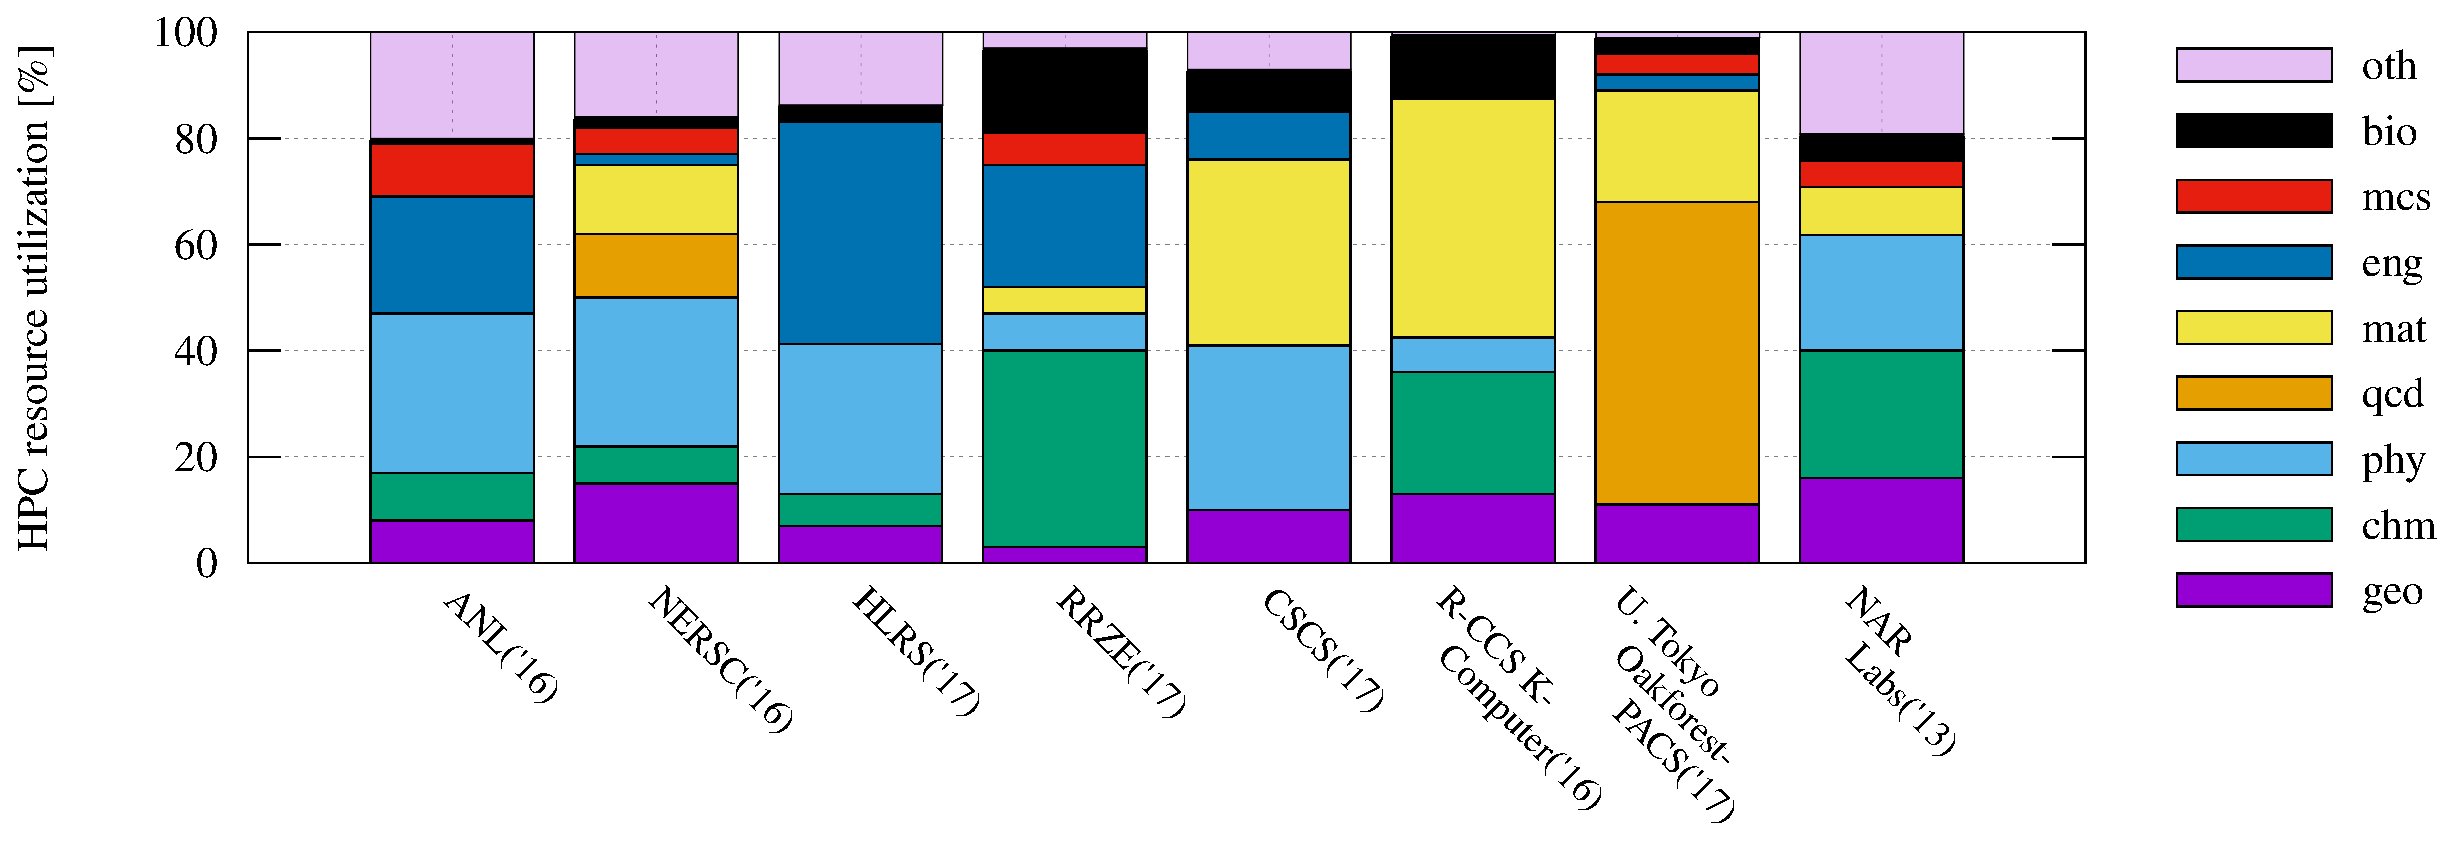
\includegraphics[width=\linewidth]{sys-util}
    \caption{\label{fid:disc:breakdown} Annual HPC site/system utilization by domain; Labels acc. to Table~\ref{table:APP}: \texttt{geo} = Geo-/Earthscience, \texttt{chm} = Chemistry, \texttt{phy} = Physics, \texttt{qcd} = Lattice QCD, \texttt{mat} = Material Science/Engineering, \texttt{eng} = Engineering (Mechanics, CFD), \texttt{mcs} = Math/Computer Science, \texttt{bio} = Bioscience, \texttt{oth} = \textit{Other}}
\end{figure}
\end{comment}
%
This paper highlights the diminishing relevance of \unit[]{flop/s} when 
considering the actual requirements of representative proxy-apps.
The relevance of \unit[]{flop/s} on a given supercomputer can be further 
diminished when considering the analysis of node-hours spent yearly on
different scientific domains at supercomputing facilities.
Figure~\ref{fid:disc:breakdown} summarizes the breakdown of node-hours by
scientific domain for different supercomputing facilities (based on yearly
reports of mentioned facilities). For instance, by simply mapping the scientific
domains in Figure~\ref{fid:disc:breakdown} to representative proxies,
ANL's ALCF and \mbox{R-CCS's} K-computer would be achieving $\approx$14\% and
$\approx$11\%, respectively, of the peak \unit[]{flop/s} when projecting
for the annual node-hours. %oversomplification?
It is worth mentioning that the relevance of \unit[]{flop/s} is even more
of an issue for supercomputers to dedicated to specific workloads: the relevance of
\unit[]{flop/s} can vary widely. For instance, a supercomputer dedicated
mainly to weather forecasting, e.g., the~\unit[18]{Pflop/s} system recently 
installed at Japan's Meteorological Agency~\cite{japan_meteorological_agency_jma_jma_2018},
should give minimal relevance to \unit[]{flop/s} since the proxy representing
this workload on that supercomputer achieves $\approx$6\% of the peak \unit[]{flop/s},
since those workloads are typically memory-bound. On the other hand, a
supercomputer dedicated to AI/ML such as ABCI, the world 5\textsuperscript{th}
fastest supercomputer as of June 2018, would put high emphasize on \unit[]{flop/s}
since deep learning workloads rely heavily on dense matrix multiplication operations.


\subsection{Memory-bound Applications}
As demonstrated in Figure~\ref{fig:flops}, the performance of memory-bound 
applications is mostly not affected by the peak \unit[]{flop/s} available. 
Accordingly, investment in data-centric architectures and programming models 
should take priority over paying premium for \unit[]{flop/s}-centric systems.
In one motivating instance, during the investigation that NASA Ames Research 
Center conducted to identify planned upgrade of the Pleiades supercomputer in 
2016~\cite{saini_performance_2016}, the study concluded that the performance gain from upgrading to
Intel Haswell processors was insignificant in comparison to using the older
Ivy Bridge-based processors (the newer processor offered double the peak
\unit[]{flop/s} at almost the same memory bandwidth). And hence the choice was only do a partial upgrade to Haswell processors.

\subsection{Compute-bound Applications}
Investing more in data-centric architectures to accommodate memory-bound 
applications can have a negative impact on the remaining minority of 
applications: compute-bound applications. Considering the market trends that
are already pushing away from dedicating the majority of chip area to
FP64 units, it is likely that libraries with compute-bound code (e.g., BLAS) 
would support mixed precision or emulation by lower precision FPUs. The 
remaining applications that do not relay on external libraries might suffer a 
performance hit. 

%\subsection{More Diversity in FPUs\cJD{not less?}}
% - option: suggest to ditch fp32 and emulate fp32 ops in fp64 units
% - mixed precision can't work (requ. hand tuning in each app) -> not practical
% - compute bound codes -> what if no FP64 anymore in new chips -> what will they do?


% - themes: time-to-solution is most important metric
% - instructions doesn't matter too much because most are memory-bound
% - apps have different requirements
% - people need to dive deeper into their workloads
% - suggestion: decouple notion of hpc apps need high FP64 and which architecture to choose => see if NASA has papers on their design choices?!
% - breakdown of node-hours on science fields across many hpc centers



% 1 page

\section{Related Work}\label{sec:relwork}
%
%\struc{alternative mini-apps, by prace, etc}
Apart from RIKEN's mini-apps and the ECP proxy-apps, which we use for our study, there are numerous benchmark suites
based on proxy applications from other HPC centers and institutes available
~\cite{prace_unified_2016,noauthor_mantevo_nodate,nersc_characterization_nodate,llnl_llnl_nodate,llnl_coral_nodate,spec_spec_nodate}.
Overall those lists show a partial overlap, either directly (i.e., same benchmark) or indirectly (same
scientific domain), between all these suites, which, for example, were used to analyze message passing characteristic~\cite{klenk_overview_2017} or to assess how predictable full application performance is
based on proxy-app measurements~\cite{barrett_assessing_2015}.
Hence, our systematic approach and published framework \textbf{\url{https://gitlab.com/domke/PAstudy}} can be
transferred to these alternative benchmarks for complementary studies, and our included raw data
can be investigated further w.r.t metrics which were outside the scope of our study.

%Scaling Deep Learning Workloads: NVIDIA DGX-1/Pascal and Intel Knights Landing: https://www.sciencedirect.com/science/article/pii/S0167739X17318599\#fig5
%Extending the Performance Analysis Tool Box: Multi-Stage CPI Stacks and FLOPS Stacks: http://heirman.net/papers/eyerman2018etpatbmscsafs.pdf 
%An Empirical Study of Intel Xeon Phi: https://arxiv.org/abs/1310.5842 
%A Novel Multi-level Integrated Roofline Model Approach for Performance Characterization: https://link.springer.com/chapter/10.1007/978-3-319-92040-5_12 
%HPC Benchmarking: Scaling Right and Looking Beyond the Average: https://link.springer.com/content/pdf/10.1007%2F978-3-319-96983-1_10.pdf 
%Pros and Cons of HPCx benchmarks: https://sc18.supercomputing.org/presentation/?id=bof107&sess=sess369 
%hot chips: Knights Landing (KNL): 2nd Generation Intel® Xeon Phi™ Processor: https://www.alcf.anl.gov/files/HC27.25.710-Knights-Landing-Sodani-Intel.pdf 
%intel's knl knm port comparison for our fig: https://www.anandtech.com/show/12172/intel-lists-knights-mill-xeon-phi-on-ark-up-to-72-cores-at-320w-with-qfma-and-vnni 
%Kernel Performance Improvement for the FEM-based Fluid Analysis Code on the K Computer: https://www.sciencedirect.com/science/article/pii/S187705091300570X
%Detecting Memory-Boundedness with Hardware Performance Counters: http://www.readex.eu/wp-content/uploads/2017/06/ICPE2017_authors_version.pdf 

\begin{comment}
\struc{similar FP studies}

\struc{other hardware directions}

\struc{alternative metrics for procurement}

\struc{studies on HPC usage categorized by science field and/or workload, such as stencils}

\struc{studies of dedicated purpose machines, such as weather, and how/why they choose certain architectures, like more memory, etc}
\end{comment}

Furthermore, the HPC community has already started to analyze relevant workloads with respect to arithmetic
intensity or memory and other potential bottlenecks for some proxy-apps~
\cite{aaziz_methodology_2018,asifuzzaman_report_2017,koskela_novel_2018}
%Aziz: https://e-reports-ext.llnl.gov/pdf/935372.pdf
%Asif: http://exanode.eu/wp-content/uploads/2017/04/D2.5.pdf
%Kosk...: https://link.springer.com/chapter/10.1007/978-3-319-92040-5_12
and individual applications~\cite{culpo_current_2012,tramm_memory_2015,kumahata_kernel_2013},
%Culpo: http://www.prace-ri.eu/IMG/pdf/Current_Bottlenecks_in_the_Scalability_of_OpenFOAM_on_Massively_Parallel_Clusters-2.pdf
%tramm: https://www.mcs.anl.gov/papers/P5056-1213.pdf
%kumaha: https://ac.els-cdn.com/S187705091300570X/1-s2.0-S187705091300570X-main.pdf?_tid=a0b19ed9-5cac-4536-9a2f-4019517d4692&acdnat=1539620006_ad61109a1b8fad4b2b17f90db5592798
revealing similar results to ours that most realistic HPC codes are not compute-bound and
achieve very low computational efficiency,
which in demonstrated cases affected procurement decisions~\cite{saini_performance_2016}.
However, to the best of our knowledge, we are the first to present a broad study across a
wide spectrum of HPC workloads which aims at characterizing bottlenecks and aims
specifically at identifying floating-point unit/precision requirements for modern architectures.

% 1/2 page

\section{Conclusion}\label{sec:conclusion}
% goal: 1/4 page
%
\struc{what did we learn which can be beneficial for others in the HPC community}

\struc{what is our recommendation for vendors and centers buying new systems}

\struc{praise our github w/ link so that others can perform similar stuff and
check, study, validate our results, also link to our TR or extended version
with appendix of less interesting results, etc.}

% 1/2 page
\iftoggle{includeacknowl}{
  \section*{Acknowledgment \& Author Contributions}
\added{
This work was supported by MEXT, JST special appointed survey 30593/2018, JST-CREST Grant Number JPMJCR1303,
JSPS KAKENHI Grant Number JP16F16764, the New Energy and Industrial Technology Development
Organization (NEDO), and the AIST/TokyoTech Real-world Big-Data Computation Open Innovation Laboratory (RWBC-OIL).
Moreover, we thank Intel for their technical support.
The authors~K.M., J.D., H.Z., K.Y., T.T. and Y.T. performed the experiments and data collection.
J.D., M.W., A.P. designed the study, analyzed the data, and supervised its execution together
with S.M., while all authors contributed to writing and editing.
}

  % 1/2 page
}{
  %
}

% references:
% 3/4 page

%\section{Introduction}
%% no \IEEEPARstart
%This demo file is intended to serve as a ``starter file''
%for IEEE conference papers produced under \LaTeX\ using
%IEEEtran.cls version 1.8b and later.
%% You must have at least 2 lines in the paragraph with the drop letter
%% (should never be an issue)
%I wish you the best of success.
%
%\hfill mds
% 
%\hfill August 26, 2015
%
%\subsection{Subsection Heading Here}
%Subsection text here.
%
%
%\subsubsection{Subsubsection Heading Here}
%Subsubsection text here.
%
%
%% An example of a floating figure using the graphicx package.
%% Note that \label must occur AFTER (or within) \caption.
%% For figures, \caption should occur after the \includegraphics.
%% Note that IEEEtran v1.7 and later has special internal code that
%% is designed to preserve the operation of \label within \caption
%% even when the captionsoff option is in effect. However, because
%% of issues like this, it may be the safest practice to put all your
%% \label just after \caption rather than within \caption{}.
%%
%% Reminder: the "draftcls" or "draftclsnofoot", not "draft", class
%% option should be used if it is desired that the figures are to be
%% displayed while in draft mode.
%%
%%\begin{figure}[!t]
%%\centering
%%\includegraphics[width=2.5in]{myfigure}
%% where an .eps filename suffix will be assumed under latex, 
%% and a .pdf suffix will be assumed for pdflatex; or what has been declared
%% via \DeclareGraphicsExtensions.
%%\caption{Simulation results for the network.}
%%\label{fig_sim}
%%\end{figure}
%
%% Note that the IEEE typically puts floats only at the top, even when this
%% results in a large percentage of a column being occupied by floats.
%
%
%% An example of a double column floating figure using two subfigures.
%% (The subfig.sty package must be loaded for this to work.)
%% The subfigure \label commands are set within each subfloat command,
%% and the \label for the overall figure must come after \caption.
%% \hfil is used as a separator to get equal spacing.
%% Watch out that the combined width of all the subfigures on a 
%% line do not exceed the text width or a line break will occur.
%%
%%\begin{figure*}[!t]
%%\centering
%%\subfloat[Case I]{\includegraphics[width=2.5in]{box}%
%%\label{fig_first_case}}
%%\hfil
%%\subfloat[Case II]{\includegraphics[width=2.5in]{box}%
%%\label{fig_second_case}}
%%\caption{Simulation results for the network.}
%%\label{fig_sim}
%%\end{figure*}
%%
%% Note that often IEEE papers with subfigures do not employ subfigure
%% captions (using the optional argument to \subfloat[]), but instead will
%% reference/describe all of them (a), (b), etc., within the main caption.
%% Be aware that for subfig.sty to generate the (a), (b), etc., subfigure
%% labels, the optional argument to \subfloat must be present. If a
%% subcaption is not desired, just leave its contents blank,
%% e.g., \subfloat[].
%
%
%% An example of a floating table. Note that, for IEEE style tables, the
%% \caption command should come BEFORE the table and, given that table
%% captions serve much like titles, are usually capitalized except for words
%% such as a, an, and, as, at, but, by, for, in, nor, of, on, or, the, to
%% and up, which are usually not capitalized unless they are the first or
%% last word of the caption. Table text will default to \footnotesize as
%% the IEEE normally uses this smaller font for tables.
%% The \label must come after \caption as always.
%%
%%\begin{table}[!t]
%%% increase table row spacing, adjust to taste
%%\renewcommand{\arraystretch}{1.3}
%% if using array.sty, it might be a good idea to tweak the value of
%% \extrarowheight as needed to properly center the text within the cells
%%\caption{An Example of a Table}
%%\label{table_example}
%%\centering
%%% Some packages, such as MDW tools, offer better commands for making tables
%%% than the plain LaTeX2e tabular which is used here.
%%\begin{tabular}{|c||c|}
%%\hline
%%One & Two\\
%%\hline
%%Three & Four\\
%%\hline
%%\end{tabular}
%%\end{table}
%
%
%% Note that the IEEE does not put floats in the very first column
%% - or typically anywhere on the first page for that matter. Also,
%% in-text middle ("here") positioning is typically not used, but it
%% is allowed and encouraged for Computer Society conferences (but
%% not Computer Society journals). Most IEEE journals/conferences use
%% top floats exclusively. 
%% Note that, LaTeX2e, unlike IEEE journals/conferences, places
%% footnotes above bottom floats. This can be corrected via the
%% \fnbelowfloat command of the stfloats package.
%
%
%
%
%\section{Conclusion}
%The conclusion goes here.
%
%
%
%
%% conference papers do not normally have an appendix
%
%
%% use section* for acknowledgment
%\section*{Acknowledgment}
%
%
%The authors would like to thank...
%
%



% trigger a \newpage just before the given reference
% number - used to balance the columns on the last page
% adjust value as needed - may need to be readjusted if
% the document is modified later
%\IEEEtriggeratref{8}
% The "triggered" command can be changed if desired:
%\IEEEtriggercmd{\enlargethispage{-5in}}

% references section

% can use a bibliography generated by BibTeX as a .bbl file
% BibTeX documentation can be easily obtained at:
% http://mirror.ctan.org/biblio/bibtex/contrib/doc/
% The IEEEtran BibTeX style support page is at:
% http://www.michaelshell.org/tex/ieeetran/bibtex/
\bibliographystyle{IEEEtran}
% argument is your BibTeX string definitions and bibliography database(s)
\bibliography{IEEEabrv,99-precision}
%
% <OR> manually copy in the resultant .bbl file
% set second argument of \begin to the number of references
% (used to reserve space for the reference number labels box)
%\begin{thebibliography}{1}
%
%\bibitem{IEEEhowto:kopka}
%H.~Kopka and P.~W. Daly, \emph{A Guide to \LaTeX}, 3rd~ed.\hskip 1em plus
%  0.5em minus 0.4em\relax Harlow, England: Addison-Wesley, 1999.
%
%\end{thebibliography}

%No appendix in first submission

\iftoggle{includeappendix}{
    \clearpage
    \appendices
%
\section{Reproducibility}\label{apx:reprod}
to infinity

\struc{code and logs in git, explain how to pull, install, compile, config, run}
\struc{explain about proprietary code and packages we dont ship with the repo}
\struc{explain how we analyze the codes, or tools/scripts we used}
\struc{detailes about software version if necessary}
\struc{have we patched any bugs? in the codes?}

\section{Detailed Input/Parameters for Benchmarks}\label{apx:inputs}
and beyond

\struc{title says it all}

\section{Additionally Evaluated Metrics}\label{apx:metrics}
woooshhhh

\struc{here comes everything text/figs/etc we left out of the main eval section}


}{
    \begin{table*}[tbp]
    \caption{\label{table:rest} Application configuration and measured metrics; Missing data for CANDLE due to SDE crashes on Phi; Measurements indicate CANDLE/MKL-DNN ignores OpenMP settings and tries to utilize full chip $\rightarrow$ listed in italic; Label explanation: t2sol = time-to-solution (kernel), Gop (D $|$ S $|$ I) = Giga operations (FP64 $|$ FP32 $|$ Integer), SIMDi/cyc = SIMD instructions per cycle, FPAIp[R $|$ W] = FP Arithmetic instructions per memory [read $|$ write], [B $|$ M]Bd = [Back-end $|$ Memory] Bound (see~\cite{sobhee_intel_2018} for details), L2h = L2 cache hit rate, LLh = Last level cache hit rate (L3 for BDW, MCDRAM for KNL/KNM), Gbra/s = Giga branches/s}%\cJD{highlight important?}}
    \centering\scriptsize
    \begin{tabular}{|l|r|r|r|r|r|r|r|c|r|r|r|r|}
        \hline \hC
        \tH{\textbf{KNL}} & \tH{\#MPI} & \tH{\#OMP} & \tH{t2sol [\unit[]{s}]} & \tH{\#Gop (D)} & \tH{\#Gop (S)} & \tH{\#Gop (I)} &  \tH{Power [\unit[]{W}]} & \tH{\#SIMDi/cyc} & \tH{BBd [\%]} & \tH{L2h [\%]} & \tH{LLh [\%]} & \tH{Gbra/s} \\ \hline
        AMG	        &	1	&	128	&	6.057	&	110.271	&	0	&	352.640	&	202.16	&	0.063	&	77.3	&	93	&    74.6	&	7.310	\\ \hline \rC
        CANDLE	    &	1	&	\textit{32}	&	59.796	&	\textit{N/A}	&	\textit{N/A}	&	\textit{N/A}	&	143.79	&	0.105	&	67.4	&	86	&    89.7	&	\textit{N/A}	\\ \hline
        CoMD	    &	32	&	8	&	3.199	&	161.691	&	14.842	&	3.476	&	189.24	&	0.077	&	81.0	&	85	&    99.4	&	11.551	\\ \hline \rC
        Laghos	    &	64	&	4	&	13.508	&	85.547	&	0.422	&	1055.977	&	143.84	&	0.021	&	23.7	&	98	&    99.7	&	7.839	\\ \hline
        MACSio	    &	64	&	1	&	35.110	&	0.613	&	0.007	&	77.884	&	140.02	&	0.002	&	52.8	&	98	&    98.6	&	18.115	\\ \hline \rC
        miniAMR	    &	128	&	1	&	47.150	&	291.536	&	0.014	&	3358.569	&	153.44	&	0.009	&	75.9	&	71	&    97.6	&	5.023	\\ \hline
        miniFE	    &	1	&	256	&	0.694	&	28.961	&	0	&	177.704	&	221.69	&	0.022	&	81.8	&	93	&    93.6	&	10.930	\\ \hline \rC
        miniTri	    &	1	&	128	&	8.630	&	0	&	0	&	118.261	&	131.49	&	0.001	&	81.9	&	66	&    99.5	&	4.531	\\ \hline
        Nekbone	    &	128	&	1	&	3.290	&	410.361	&	0	&	23.371	&	221.48	&	0.050	&	76.5	&	87	&    97.6	&	6.125	\\ \hline \rC
        SW4lite	    &	64	&	4	&	1.686	&	145.938	&	0	&	0.761	&	214.57	&	0.096	&	80.6	&	95	&    98.4	&	2.218	\\ \hline
        SWFFT	    &	128	&	1	&	1.235	&	12.688	&	0.005	&	42.509	&	174.12	&	0.029	&	76.7	&	83	&    98.6	&	20.905	\\ \hline \rC
        XSBench	    &	1	&	256	&	1.290	&	27.283	&	0.417	&	16.441	&	192.46	&	0.041	&	93.7	&	22	&    99.5	&	2.629	\\ \hline\hline
        FFB	        &	64	&	2	&	8.244	&	2.300	&	258.561	&	1785.716	&	179.55	&	0.159	&	38.4	&	89	&    99.7	&	2.717	\\ \hline \rC
        FFVC	    &	1	&	64	&	13.009	&	134.589	&	1579.917	&	20174.483	&	180.58	&	0.169	&	36.0	&	95	&    99.7	&	4.415	\\ \hline
        mVMC	    &	32	&	6	&	20.679	&	1141.865	&	1.345	&	1746.001	&	180.98	&	0.036	&	81.9	&	91	&    98.9	&	6.073	\\ \hline \rC
        MODYLAS	    &	64	&	4	&	22.514	&	6287.279	&	2.063	&	23104.728	&	206.98	&	0.072	&	80.4	&	97	&    95.7	&	7.742	\\ \hline
        NGSA	    &	4	&	32	&	829.675	&	0.826	&	0.023	&	69.117	&	97.91	&	0.002	&	51.9	&	71	&    95.9	&	1.050	\\ \hline \rC
        NICAM	    &	10	&	15	&	37.802	&	422.504	&	0.066	&	925.228	&	119.46	&	0.193	&	67.8	&	92	&    99.2	&	0.231	\\ \hline
        NTChem	    &	16	&	8	&	18.985	&	1629.210	&	0.627	&	2303.804	&	167.13	&	0.060	&	64.4	&	91	&    99.2	&	5.429	\\ \hline \rC
        QCD	        &	1	&	128	&	8.437	&	631.522	&	0	&	3823.335	&	215.67	&	0.220	&	69.4	&	88	&    95.4	&	1.151	\\ \hline\hline
        HPCG	    &	96	&	1	&	44.612	&	612.799	&	0	&	17530.136	&	181.69	&	0.023	&	86.1	&	91	&    45.7	&	1.446	\\ \hline \rC
        HPL	        &	64	&	1	&	145.400	&	184191.774	&	0.015	&	20226.567	&	221.13	&	0.374	&	52.3	&	93	&    87.9	&	1.232	\\ \hline
        \hline \hC
        \tH{\textbf{KNM}} & \tH{\#MPI} & \tH{\#OMP} & \tH{t2sol [\unit[]{s}]} & \tH{\#Gop (D)} & \tH{\#Gop (S)} & \tH{\#Gop (I)} &  \tH{Power [\unit[]{W}]} & \tH{\#SIMDi/cyc} & \tH{BBd [\%]} & \tH{L2h [\%]} & \tH{LLh [\%]} & \tH{Gbra/s} \\ \hline
        AMG	        &	1	&	128	&	7.434	&	110.271	&	0	&	352.639	&	202.52	&	0.062	&	75.4	&	94	&   73.3	&	6.392	\\ \hline \rC
        CANDLE	    &	1	&	\textit{144}	&	50.527	&	\textit{N/A}	&	\textit{N/A}	&	\textit{N/A}	&	153.69	&	0.040	&	82.4	&	92	&	90.9	&	\textit{N/A}	\\ \hline
        CoMD	    &	72	&	2	&	3.194	&	161.842	&	14.880	&	3.479	&	196.64	&	0.177	&	67.5	&	86	&	99.1	&	11.546	\\ \hline \rC
        Laghos	    &	64	&	4	&	12.725	&	85.383	&	0.422	&	1056.141	&	139.33	&	0.023	&	25.1	&	98	&	99.8	&	8.345	\\ \hline
        MACSio	    &	64	&	1	&	33.236	&	0.613	&	0.007	&	77.884	&	135.48	&	0.002	&	53.8	&	98	&	98.2	&	19.206	\\ \hline \rC
        miniAMR	    &	128	&	1	&	44.653	&	291.536	&	0.014	&	3358.570	&	177.31	&	0.009	&	75.3	&	71	&	97.3	&	5.337	\\ \hline
        miniFE	    &	72	&	1	&	0.669	&	32.892	&	0	&	669.371	&	210.18	&	0.097	&	55.6	&	60	&	98.3	&	7.393	\\ \hline \rC
        miniTri	    &	1	&	128	&	9.545	&	0	&	0	&	118.262	&	122.02	&	0	&	80.9	&	68	&	99.6	&	4.102	\\ \hline
        Nekbone	    &	144	&	1	&	2.984	&	410.381	&	0	&	23.470	&	233.46	&	0.040	&	76.1	&	87	&	96.6	&	6.494	\\ \hline \rC
        SW4lite	    &	72	&	4	&	1.569	&	146.048	&	0	&	0.764	&	228.01	&	0.090	&	81.3	&	96	&	97.8	&	2.753	\\ \hline
        SWFFT	    &	128	&	1	&	1.189	&	12.555	&	0.005	&	41.732	&	172.66	&	0.026	&	77.2	&	83	&	98.5	&	21.990	\\ \hline \rC
        XSBench	    &	1	&	288	&	1.220	&	30.603	&	0.417	&	16.440	&	197.16	&	0.038	&	91.5	&	22	&	98.5	&	2.783	\\ \hline\hline
        FFB	        &	64	&	2	&	7.750	&	2.300	&	258.565	&	1785.712	&	178.72	&	0.171	&	38.6	&	89	&	99.7	&	2.886	\\ \hline \rC
        FFVC	    &	1	&	72	&	13.497	&	134.589	&	1579.917	&	20174.587	&	182.05	&	0.162	&	55.2	&	94	&	99.9	&	5.055	\\ \hline
        mVMC	    &	72	&	4	&	19.659	&	1140.670	&	1.347	&	1802.663	&	197.64	&	0.012	&	76.0	&	91	&	98.5	&	8.869	\\ \hline \rC
        MODYLAS	    &	64	&	4	&	24.026	&	6287.279	&	2.063	&	23104.728	&	217.47	&	0.062	&	80.0	&	97	&	95.6	&	7.153	\\ \hline
        NGSA	    &	4	&	18	&	724.546	&	0.826	&	0.023	&	69.300	&	88.67	&	0.002	&	39.5	&	68	&	94.9	&	1.138	\\ \hline \rC
        NICAM	    &	10	&	7	&	34.380	&	422.504	&	0.066	&	925.229	&	113.88	&	0.208	&	68.2	&	92	&	99.1	&	0.248	\\ \hline
        NTChem	    &	72	&	2	&	14.606	&	1575.310	&	0.623	&	1985.255	&	176.51	&	0.066	&	59.0	&	90	&	98.4	&	7.038	\\ \hline \rC
        QCD	        &	1	&	144	&	9.662	&	631.522	&	0	&	3823.337	&	200.86	&	0.175	&	72.6	&	88	&	95.9	&	2.121	\\ \hline\hline
        HPCG	    &	64	&	1	&	42.865	&	612.605	&	0	&	17532.326	&	174.58	&	0.041	&	86.5	&	95	&   42.9	&	2.878	\\ \hline \rC
        HPL	        &	72	&	1	&	146.562	&	184893.073	&	0.016	&	20414.548	&	263.59	&	0.351	&	57.0	&	92	&   87.0	&	1.885	\\ \hline
        \hline \hC
        \tH{\textbf{BDW}} & \tH{\#MPI} & \tH{\#OMP} & \tH{t2sol [\unit[]{s}]} & \tH{\#Gop (D)} & \tH{\#Gop (S)} & \tH{\#Gop (I)} & \tH{Power [\unit[]{W}]} & \tH{FPAIp[R : W]} & \textcolor{white}{MBd [\%]} & \tH{L2h [\%]} & \tH{LLh [\%]} & \tH{Gbra/s} \\ \hline
        AMG	        &	8	&	6	&	10.780	&	110.810	&	0	&	362.209	&	152.21	&	0.361 : 5.516	&	44.8	&	21		&	17  &	4.354	\\ \hline \rC
        CANDLE	    &	1	&	\textit{12}	&	78.240	&	0.012	&	6918.340	&	2783.532	&	132.38	&	1.078 : 2.800	&	26.7	&	23		&    11	&	1.242	\\ \hline
        CoMD	    &	48	&	1	&	2.921	&	152.022	&	0	&	0.205	&	133.17	&	0.845 : 6.615	&	1.5		&	15		&    15	&	11.391	\\ \hline \rC
        Laghos	    &	24	&	1	&	5.5472	&	44.534	&	0	&	421.465	&	126.51	&	0.184 : 0.476	&	13.2	&	81		&    56	&	16.808	\\ \hline
        MACSio	    &	4	&	1	&	10.498	&	0.070	&	0	&	72.582	&	89.3	&	0 : 0	&	0.8		&	48		&    59	&	3.274	\\ \hline \rC
        miniAMR	    &	96	&	1	&	55.386	&	40.816	&	0	&	172.317	&	133.29	&	0.059 : 0.311	&	55.1	&	24		&    23	&	4.013	\\ \hline
        miniFE	    &	24	&	1	&	1.475	&	30.693	&	0	&	120.715	&	152.77	&	0.311 : 5.454	&	55.2	&	15		&    12	&	4.699	\\ \hline \rC
        miniTri	    &	1	&	48	&	5.478	&	0	&	0	&	118.178	&	112.61	&	0 : 0	&	34.0	&	47		&	90    &	7.106	\\ \hline
        Nekbone	    &	96	&	1	&	5.671	&	301.559	&	0	&	10.139	&	154.74	&	0.593 : 2.431	&	36.9	&	36		&	24    &	3.915	\\ \hline \rC
        SW4lite	    &	24	&	2	&	2.056	&	136.835	&	0	&	1.585	&	146.65	&	1.044 : 4.580	&	9.1		&	75		&    18	&	1.112	\\ \hline
        SWFFT	    &	32	&	1	&	1.088	&	12.239	&	0	&	38.782	&	134.55	&	0.117 : 0.675	&	28.3	&	23		&    32	&	20.932	\\ \hline \rC
        XSBench	    &	1	&	96	&	2.022	&	19.921	&	0	&	20.280	&	132.25	&	0.807 : 3.847	&	71.7	&	5		&    18	&	1.653	\\ \hline\hline
        FFB	        &	24	&	1	&	5.327	&	1.300	&	233.640	&	2116.421	&	144.35	&	0.635 : 2.200	&	21.3	&	79		&    33	&	3.723	\\ \hline \rC
        FFVC	    &	12	&	4	&	12.691	&	127.322	&	1573.782	&	27857.376	&	151.85	&	0.481 : 2.844	&	3.3		&	84		&    57	&	9.045	\\ \hline
        mVMC	    &	24	&	2	&	13.489	&	1092.394	&	0	&	2224.092	&	152.28	&	0.601 : 2.456	&	12.0	&	36		&    24	&	10.170	\\ \hline \rC
        MODYLAS	    &	16	&	3	&	36.101	&	5363.366	&	0	&	10888.745	&	135.75	&	0.875 : 8.736	&	8.1		&	60		&    31	&	5.385	\\ \hline
        NGSA	    &	12	&	4	&	105.879	&	0.826	&	0.023	&	64.249	&	107.15	&	0.002 : 0.006	&	6.5		&	21		&    36	&	8.566	\\ \hline \rC
        NICAM	    &	10	&	6	&	28.449	&	428.282	&	0.003	&	687.852	&	118.32	&	0.540 : 3.732	&	49.6	&	27		&    19	&	0.585	\\ \hline
        NTChem	    &	24	&	1	&	8.963	&	1315.509	&	0	&	778.829	&	141.3	&	0.867 : 4.931	&	9.4		&	56		&    39	&	10.173	\\ \hline \rC
        QCD	        &	1	&	24	&	13.102	&	612.303	&	0	&	3817.944	&	153.2	&	1.152 : 4.542	&	45.2	&	27		&    24	&	0.368	\\ \hline\hline
        HPCG	    &	2	&	24	&	38.595	&	559.046	&	0	&	90.171	&	166.18	&	0.143 : 0.628	&	11.3	&	34		&    23		&	10.928	\\ \hline \rC
        HPL	        &	24	&	1	&	271.794	&	181484.240	&	0	&	31919.479	&	189.37	&	\,~~2.280 : 122.693	&	3.9		&	10		&    3    	&	2.147	\\ \hline
    \end{tabular}
\end{table*}

}

% that's all folks
\end{document}
